\documentclass{article}
\usepackage[utf8]{inputenc}
\usepackage[greek,english]{babel}
\usepackage{alphabeta}
\usepackage{graphicx}
\usepackage{hyperref} 
\usepackage{listings}
\usepackage{subcaption}
\usepackage{mathtools}
\usepackage{amsmath}

\date{\vspace{-4ex}}
\title{Συστήματα Μικροϋπολογιστών}
\usepackage[svgnames]{xcolor} 
\newcommand*{\plogo}{\fbox{$\mathcal{PL}$}} 
\begin{document}

\begin{titlepage} % Suppresses displaying the page number on the title page and the subsequent page counts as page 1
	
	\raggedleft % Right align the title page
	
	\rule{1pt}{\textheight} % Vertical line
	\hspace{0.05\textwidth} % Whitespace between the vertical line and title page text
	\parbox[b]{0.75\textwidth}{ % Paragraph box for holding the title page text, adjust the width to move the title page left or right on the page
		
		{\Huge\bfseries Δίκτυα \\[0.5\baselineskip] Υπολογιστών ΙI}\\[2\baselineskip] % Title
		{\large\textit{ }}\\[4\baselineskip] % Subtitle or further description
		{\Large\textsc{Ιωάννης-Παναγιώτης \\Μπουντουρίδης}} %
	\\	\\{\large\textsc{ΑΕΜ: 8872}} % Author name, lower case for consistent small caps
		
		\vspace{0.5\textheight} % Whitespace between the title block and the publisher
		
		{\noindent \textit{session 1}}\\[\baselineskip] % Publisher and logo
	}

\end{titlepage}

\newpage
\large{}
\section*{G1. Χρόνος απόκρισης συστήματος}
Στο γράφημα που ακολουθεί εμφανίζουμε, για χρονική διάρκεια 5 λεπτών, το χρόνο απόκρισης του
συστήματος σε milliseconds για κάθε πακέτο echo που έχει αποσταλεί στην διάρκεια της συνεδρίας.

\begin{figure*}[h!]
 \begin{center}
 \advance\leftskip-4cm
  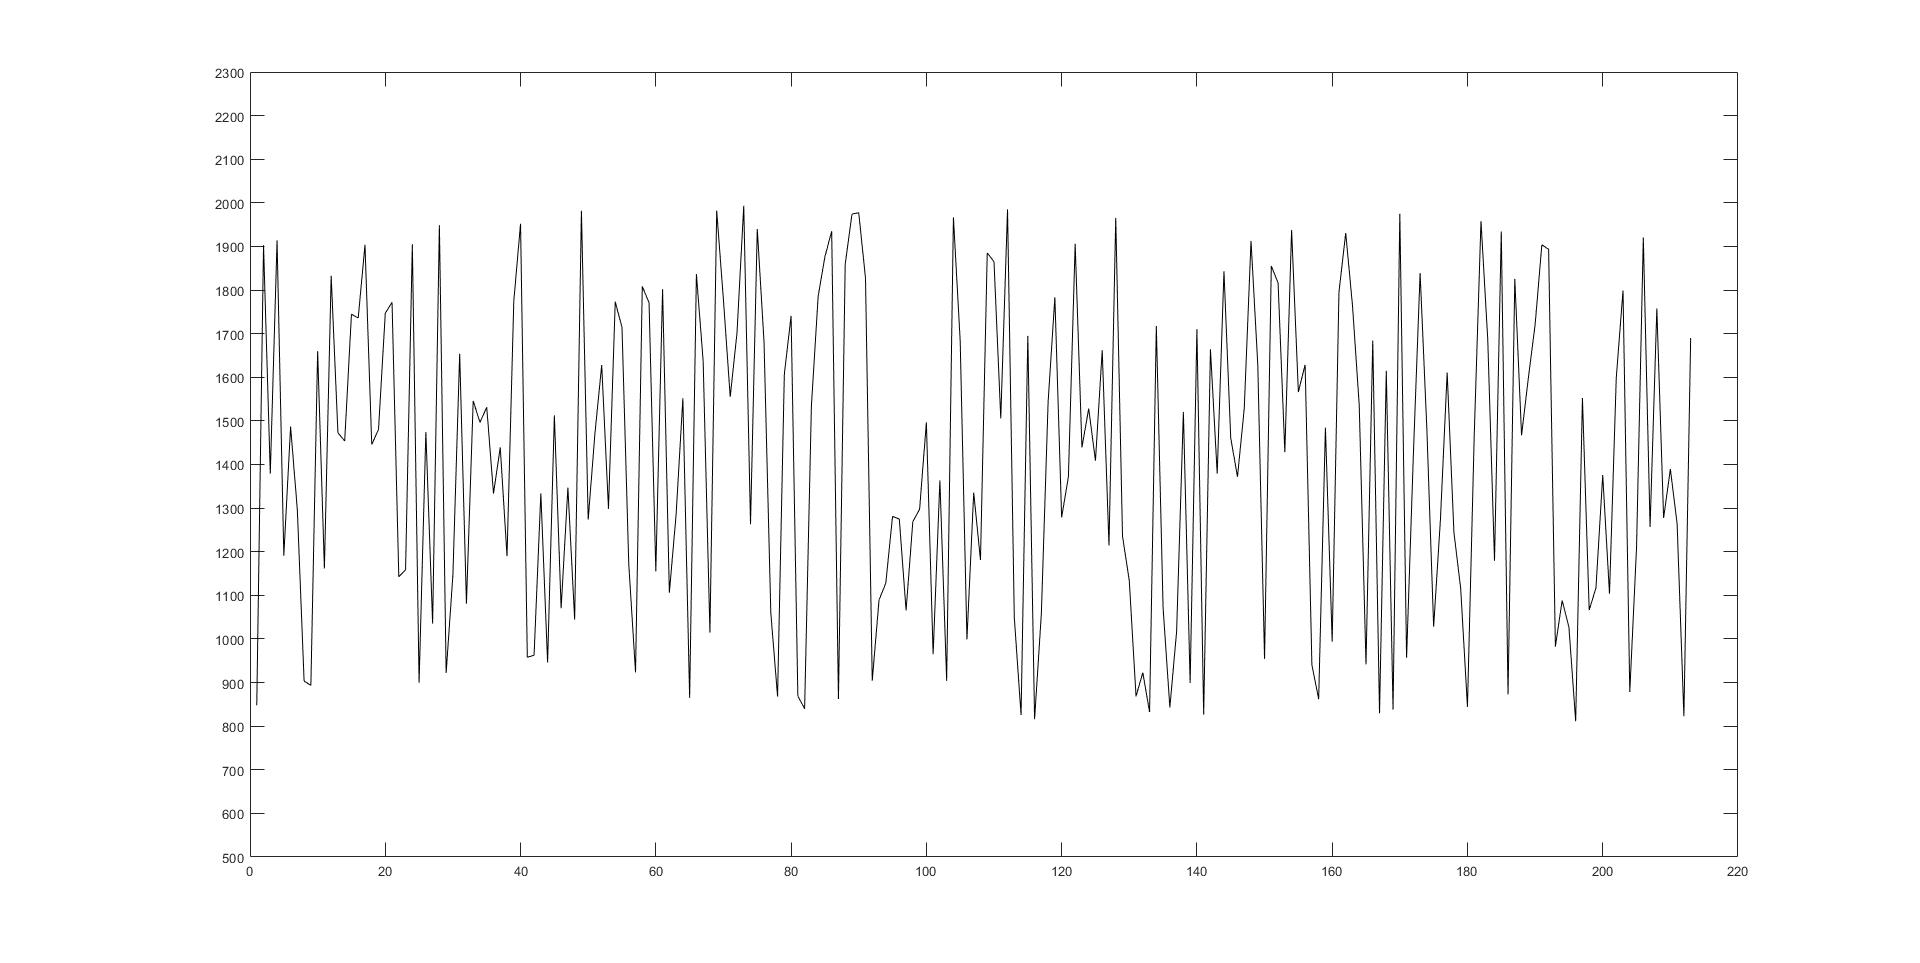
\includegraphics[width=200mm,scale=0.7]{g1s1.jpg}
  \caption*{\textbf{echo packets with delay}}
  
\end{center}
\end{figure*}
\paragraph{Διάρκεια συνεδρίας:} 5 λεπτα
\paragraph{Συνολικός αριθμός πακέτων: }213
\paragraph{Μέσος χρόνος απόκρισης: }1411 ms
\newpage
\large{}
\section*{G2. Ρυθμαπόδοση συστήματος (throughput)}
Στο γράφημα που ακολουθεί εμφανίζουμε, για χρονική διάρκεια 5 λεπτών, τη ρυθμαπόδοση (throughput) του συστήματος υπολογιζόμενη με
την τεχνική του κινούμενου μέσου όρου κάθε δευτερόλεπτο για τα 8 πλέον πρόσφατα δευτερόλεπτα κάθε φορά.

\begin{figure*}[h!]
 \begin{center}
  \advance\leftskip-6cm
  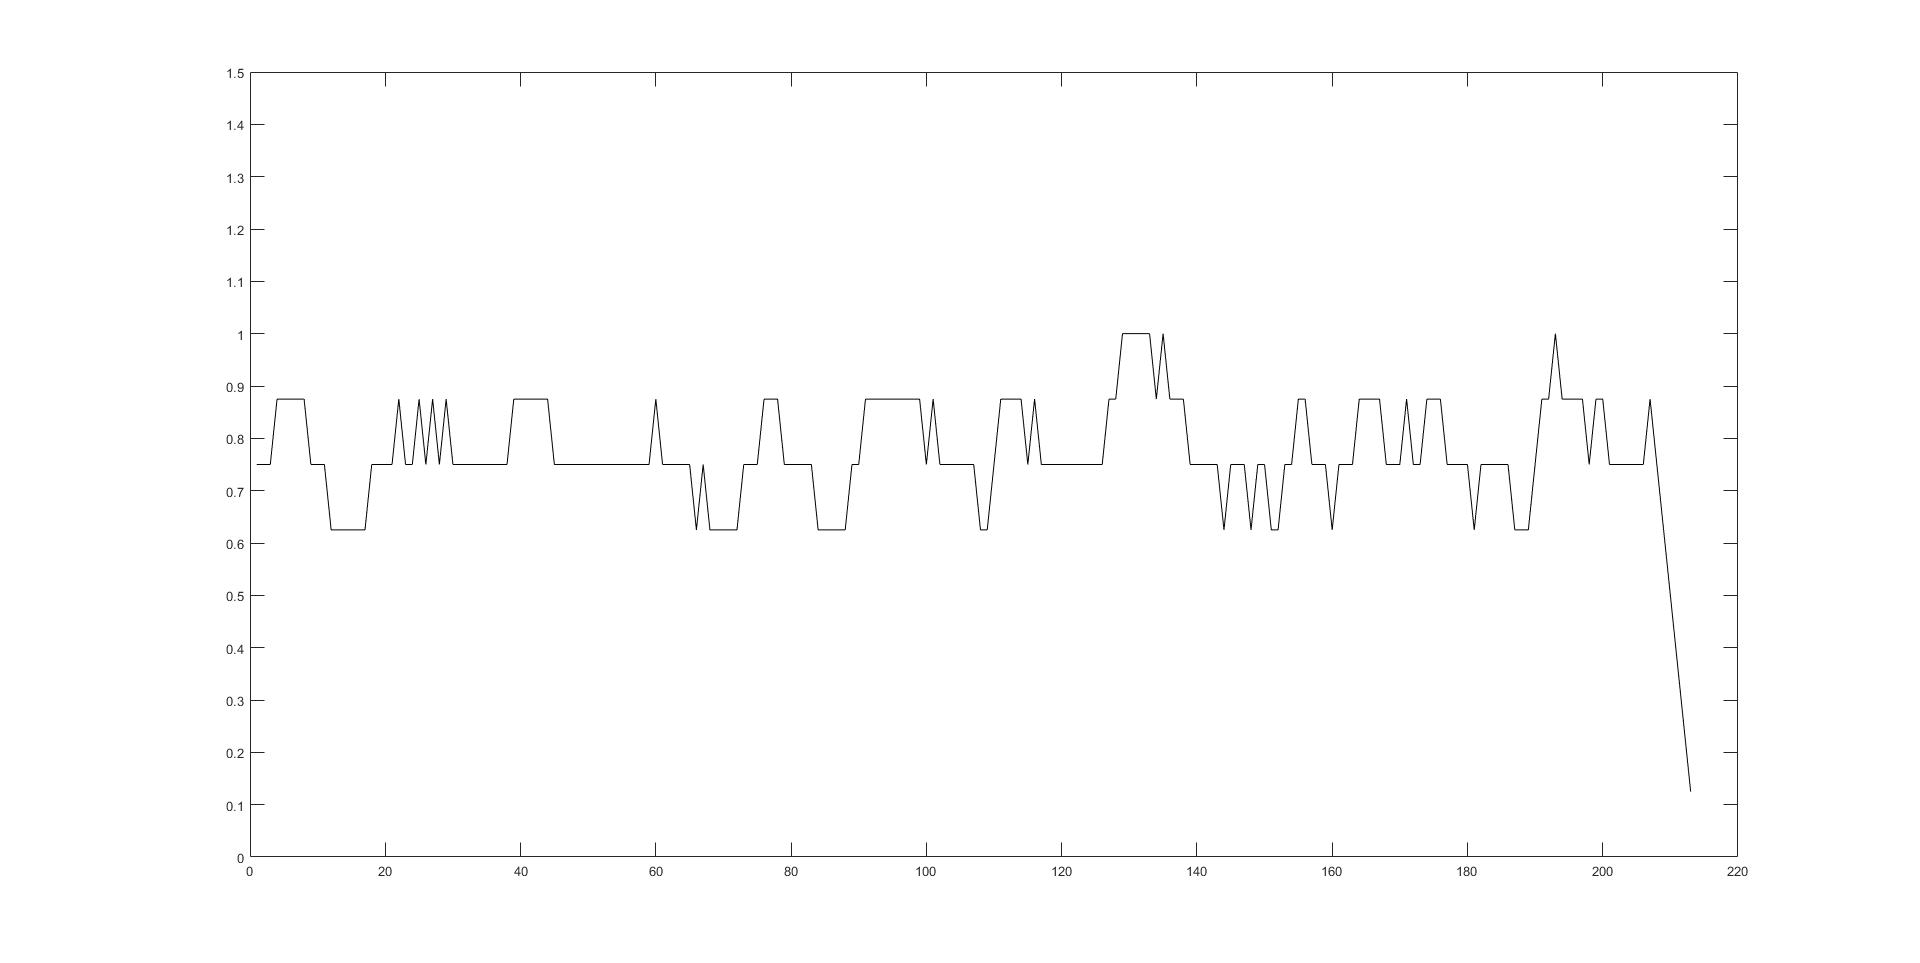
\includegraphics[width=240mm,scale=0.7]{g2s1.jpg}
    \caption*{\textbf{echo packets with delay}}
  
\end{center}
\end{figure*}
\paragraph{Διάρκεια συνεδρίας:} 5 λεπτα
\newpage
\large{}
\section*{G3. Χρόνος απόκρισης συστήματος}
Στο γράφημα που ακολουθεί εμφανίζουμε, για χρονική διάρκεια 5 λεπτών, το χρόνο απόκρισης του
συστήματος σε milliseconds για κάθε πακέτο echo που έχει αποσταλεί στην διάρκεια της συνεδρίας.

\begin{figure*}[h!]
 \begin{center}
 \advance\leftskip-4cm
  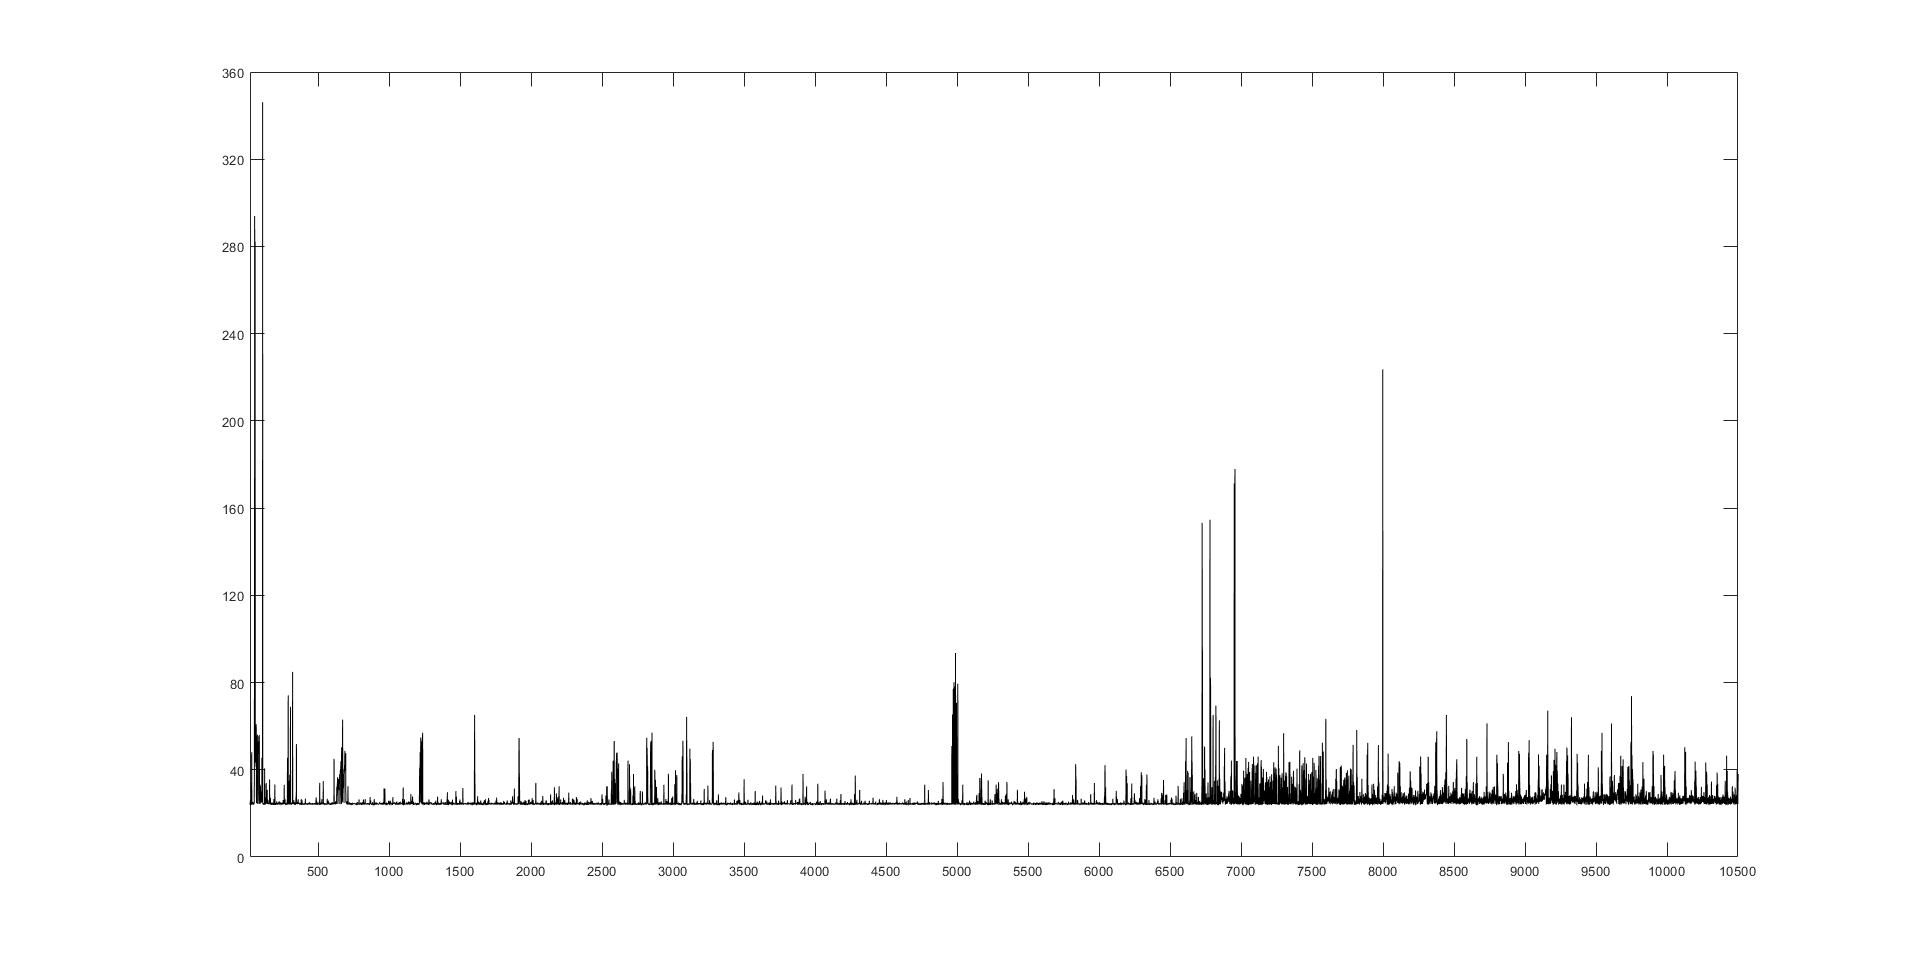
\includegraphics[width=200mm,scale=0.7]{g3s1.jpg}
  \caption*{\textbf{echo packets without delay}}
  
\end{center}
\end{figure*}
\paragraph{Διάρκεια συνεδρίας:} 5 λεπτα
\paragraph{Συνολικός αριθμός πακέτων: }10681
\paragraph{Μέσος χρόνος απόκρισης: }26 ms
\newpage
\large{}
\section*{G4. Ρυθμαπόδοση συστήματος (throughput)}
Στο γράφημα που ακολουθεί εμφανίζουμε, για χρονική διάρκεια 5 λεπτών, τη ρυθμαπόδοση (throughput) του συστήματος υπολογιζόμενη με
την τεχνική του κινούμενου μέσου όρου κάθε δευτερόλεπτο για τα 8 πλέον πρόσφατα δευτερόλεπτα κάθε φορά.

\begin{figure*}[h!]
 \begin{center}
 \advance\leftskip-6cm
  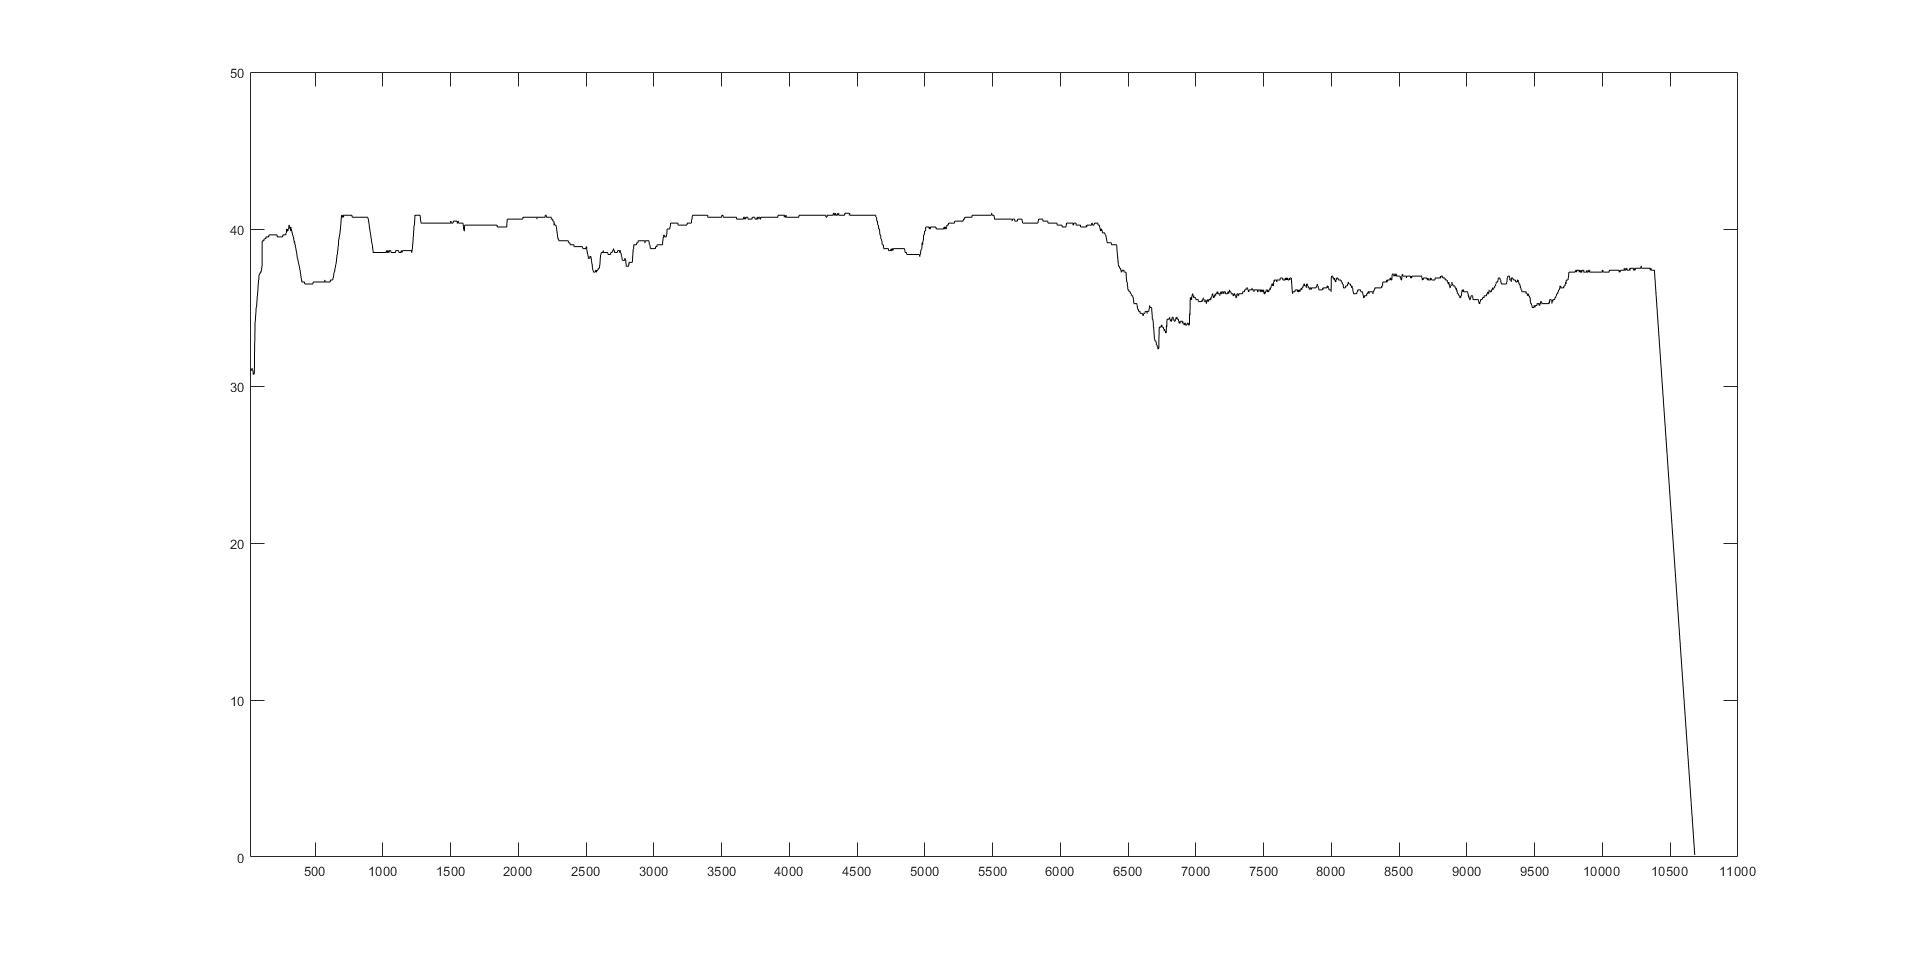
\includegraphics[width=240mm,scale=0.7]{g4s1.jpg}
   \caption*{\textbf{echo packets without delay}}
  
\end{center}
\end{figure*}
\paragraph{Διάρκεια συνεδρίας:} 5 λεπτα
\newpage
\large{}

\section*{G5. Ιστόγραμμα χρόνου απόκρισης}

\begin{figure*}[h!]
 \begin{center}
 \advance\leftskip-2.3cm
  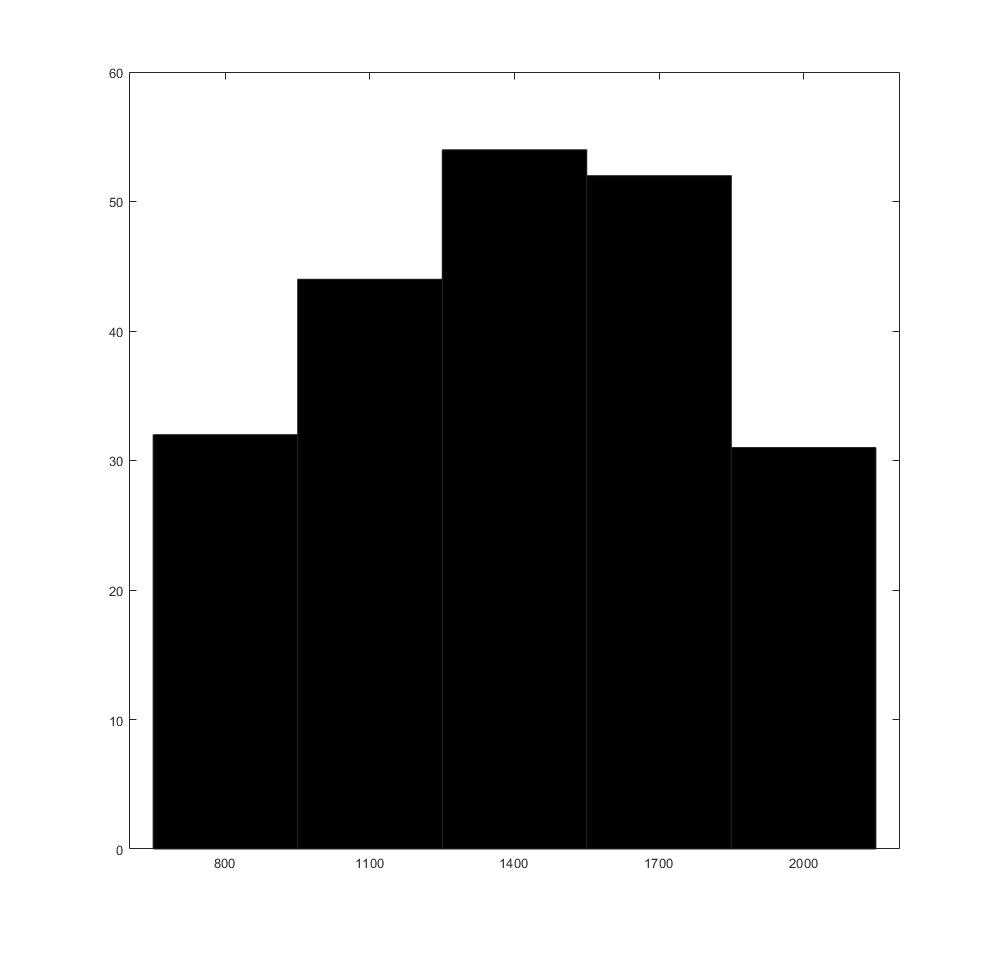
\includegraphics[width=160mm,scale=0.7]{g5s1.jpg}
    \caption*{\textbf{echo packets with delay}}
  
\end{center}
\end{figure*}
\paragraph{Διάρκεια συνεδρίας:} 5 λεπτα
\newpage
\large{}

\section*{G6. Ιστόγραμμα  ρυθμαπόδοσης για 8 δευτερόλεπτα}

\begin{figure*}[h!]
 \begin{center}
 \advance\leftskip-6.8cm
  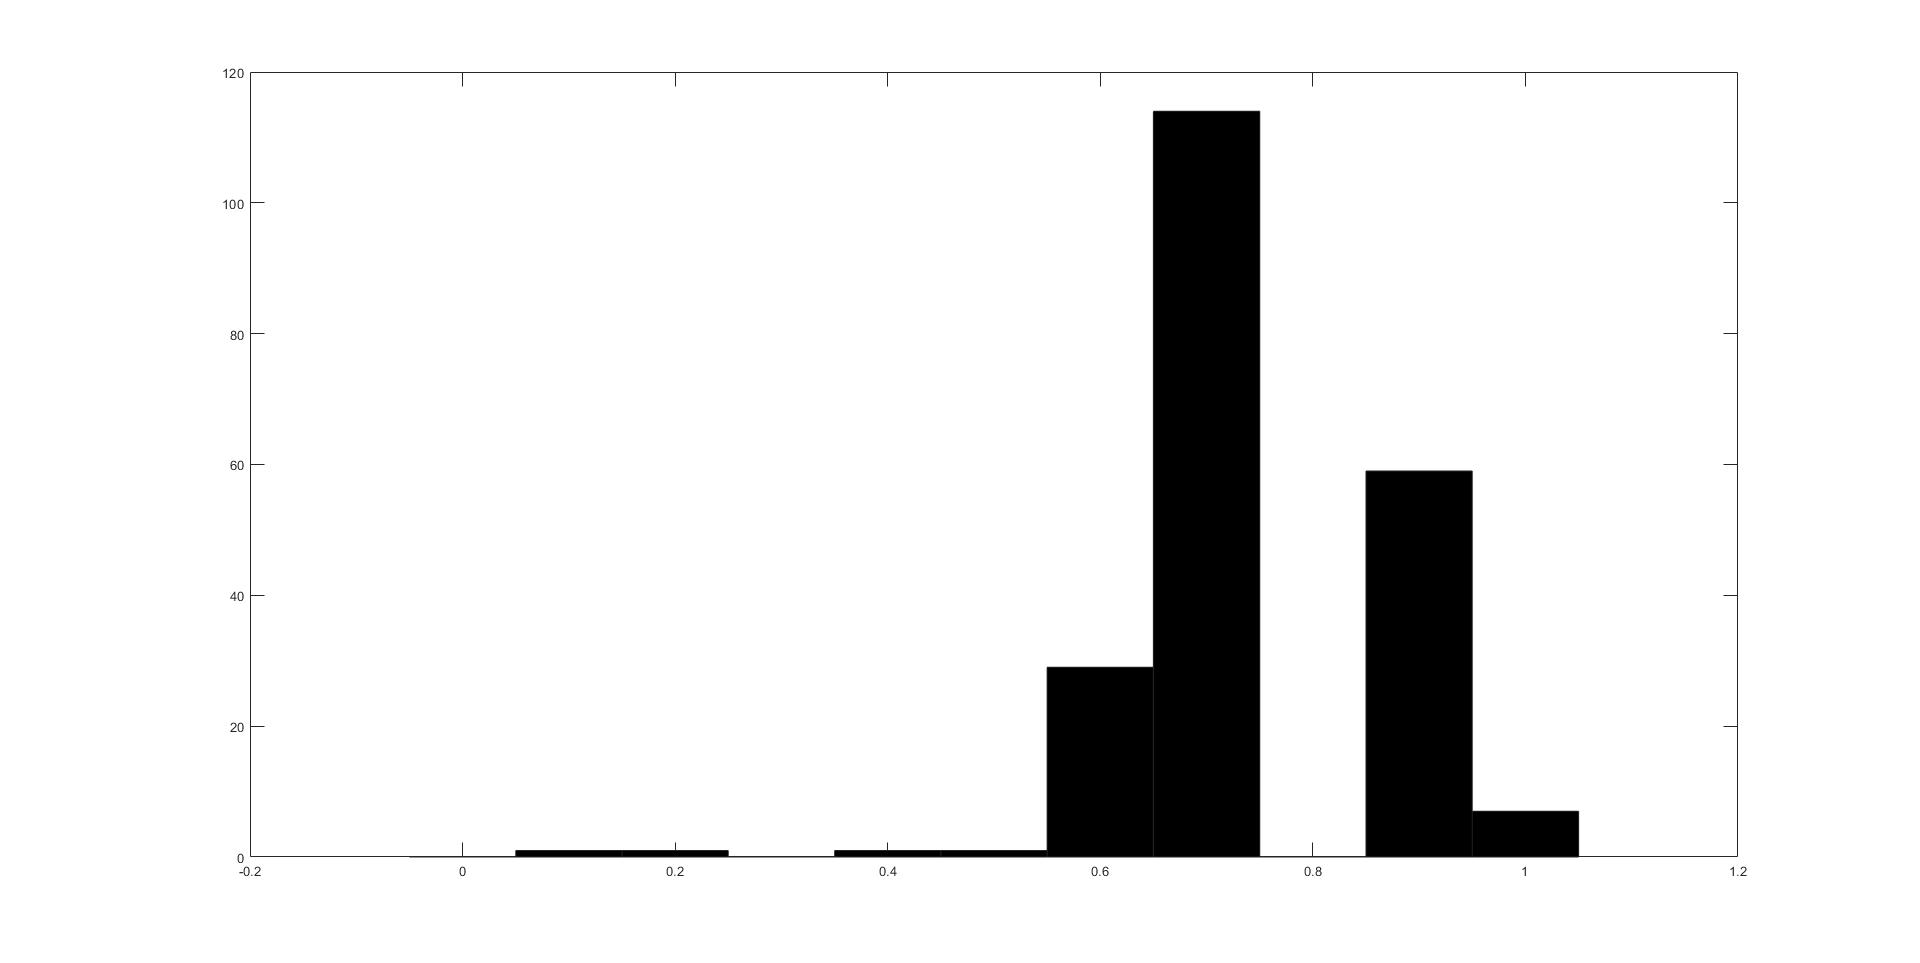
\includegraphics[width=250mm,scale=0.7]{g6s1.jpg}
    \caption*{\textbf{echo packets with delay}}
  
\end{center}
\end{figure*}
\paragraph{Διάρκεια συνεδρίας:} 5 λεπτα
\newpage
\large{}

\section*{G7. Ιστόγραμμα χρόνου απόκρισης}

\begin{figure*}[h!]
 \begin{center}
 \advance\leftskip-6.8cm
  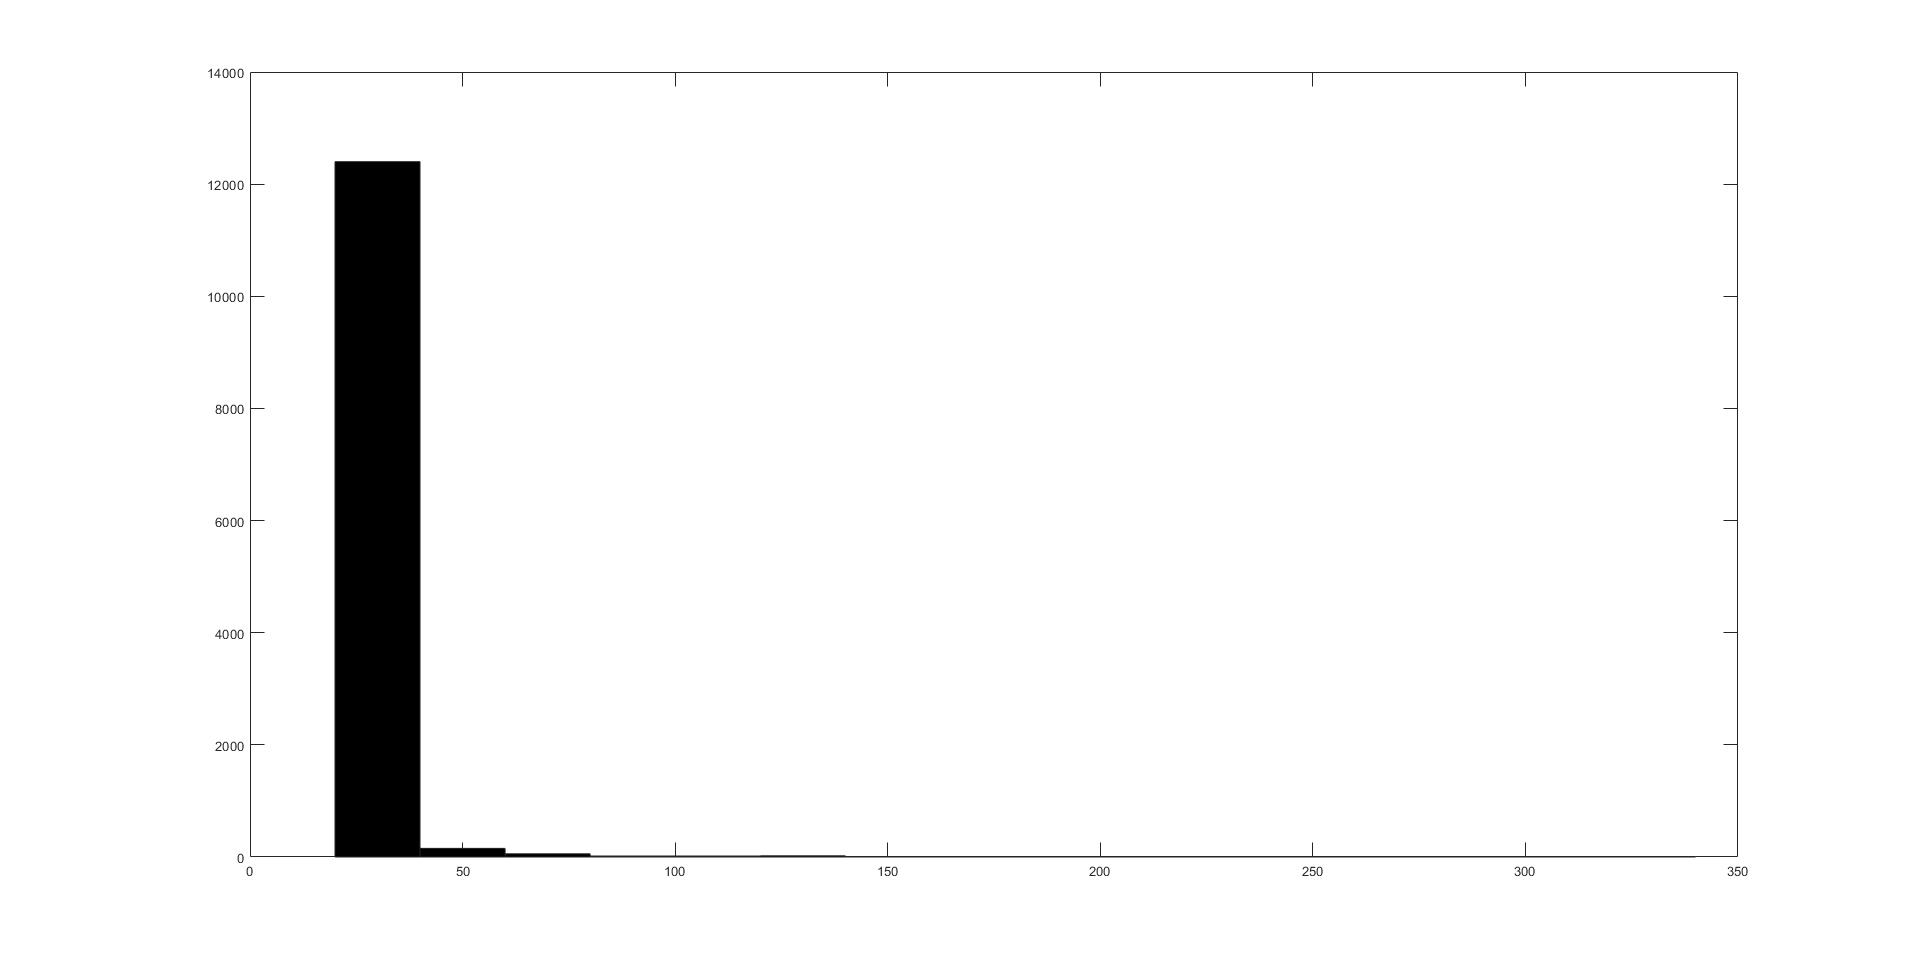
\includegraphics[width=250mm,scale=0.7]{g7s1.jpg}
    \caption*{\textbf{echo packets without delay}}
  
\end{center}
\end{figure*}
\paragraph{Διάρκεια συνεδρίας:} 5 λεπτα
\newpage
\large{}

\section*{G8. Ιστόγραμμα ρυθμαπόδοσης για 8 δευτερόλεπτα}

\begin{figure*}[h!]
 \begin{center}
 \advance\leftskip-6.8cm
  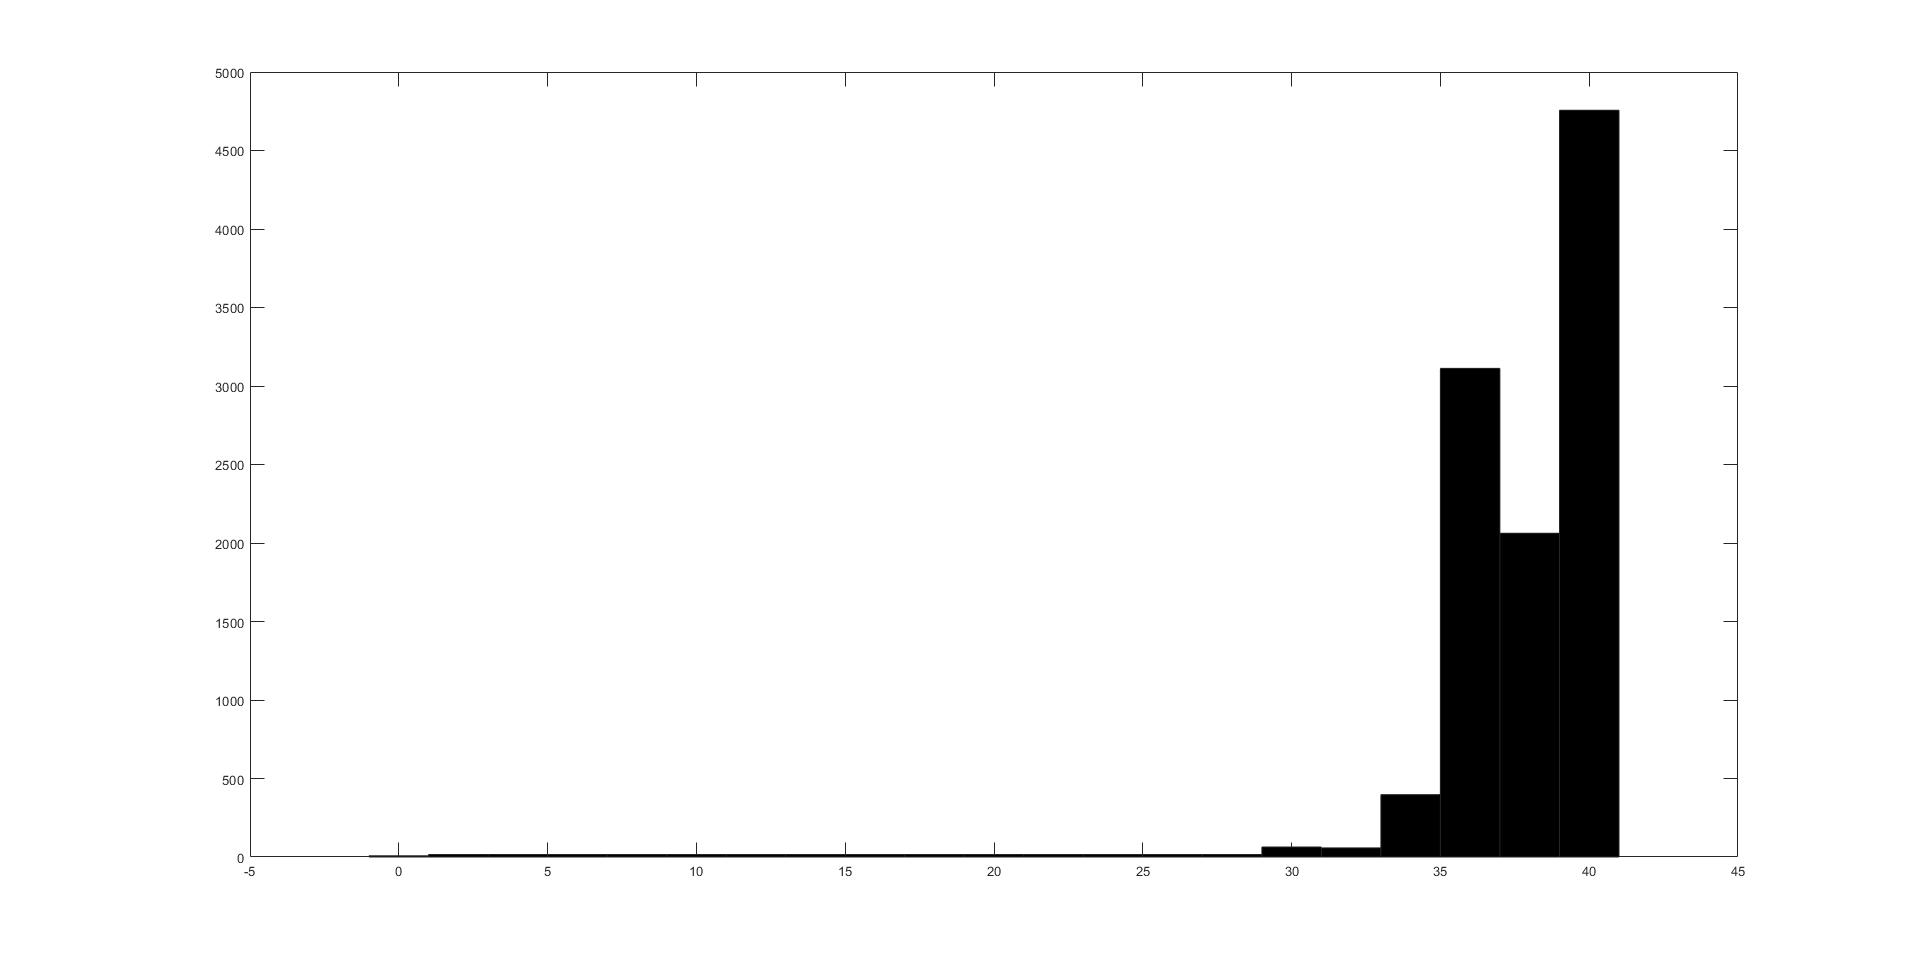
\includegraphics[width=250mm,scale=0.7]{g8s1.jpg}
    \caption*{\textbf{echo packets without delay}}
  
\end{center}
\end{figure*}
\paragraph{Διάρκεια συνεδρίας:} 5 λεπτα
\newpage
\large{}

\section*{E1. CAMERA 1}

\begin{figure*}[h!]
 \begin{center}
 \advance\leftskip-4cm
  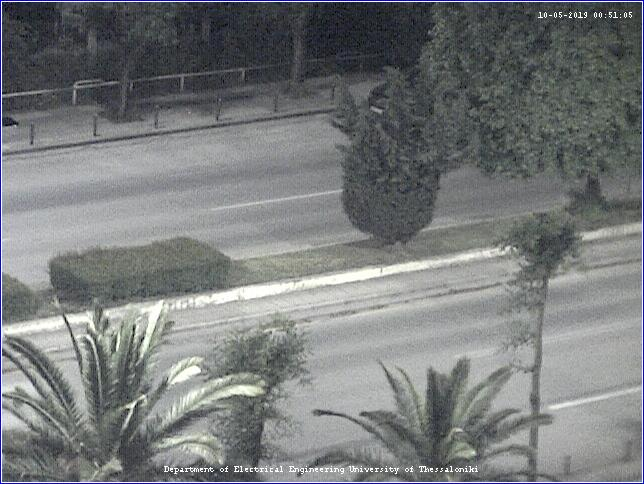
\includegraphics[width=200mm,scale=0.7]{pic1s1.jpeg}
   
  
\end{center}
\end{figure*}
\newpage
\large{}

\section*{E2. CAMERA 2}

\begin{figure*}[h!]
 \begin{center}
 \advance\leftskip-4cm
  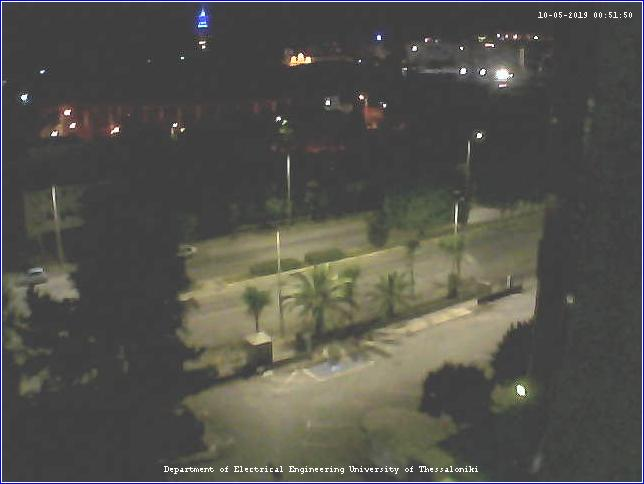
\includegraphics[width=200mm,scale=0.7]{pic2s1.jpeg}
   
  
\end{center}
\end{figure*}
\newpage
\section*{Θερμοκρασίες}
\textbf{Τ1.} PSTART 10-05-2019 00:53:52 T00 10-05 00:53 +26 C PSTOP
\section*{G9. Διάγραμμα απο την εικονική γεννήτρια συχνοτήτων (DPCM)}
\begin{figure*}[h!]
 \begin{center}
 \advance\leftskip-4cm
  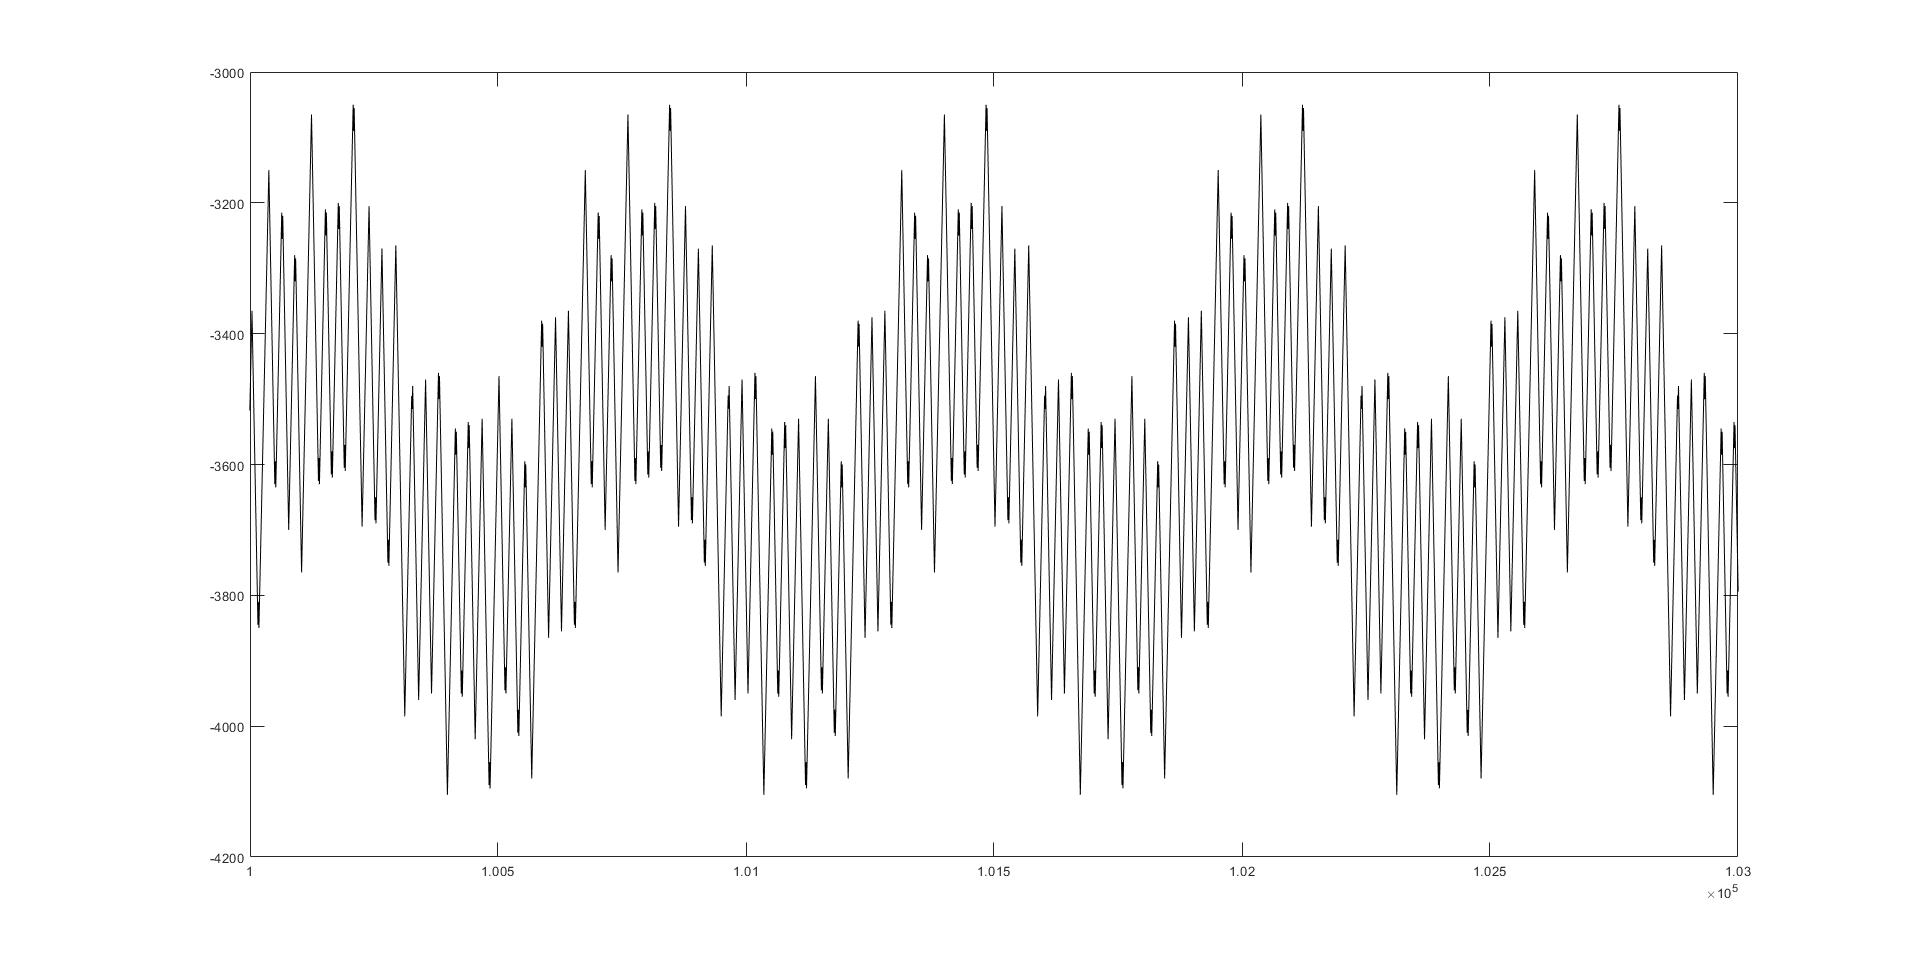
\includegraphics[width=200mm,scale=0.7]{g9s1.jpg}
\end{center}
\end{figure*}
\newpage
\section*{Τραγούδι: Chase the sun}
\section*{G10. Διάγραμμα δειγμάτων (DPCM) }
\begin{figure*}[h!]
 \begin{center}
 \advance\leftskip-6cm
  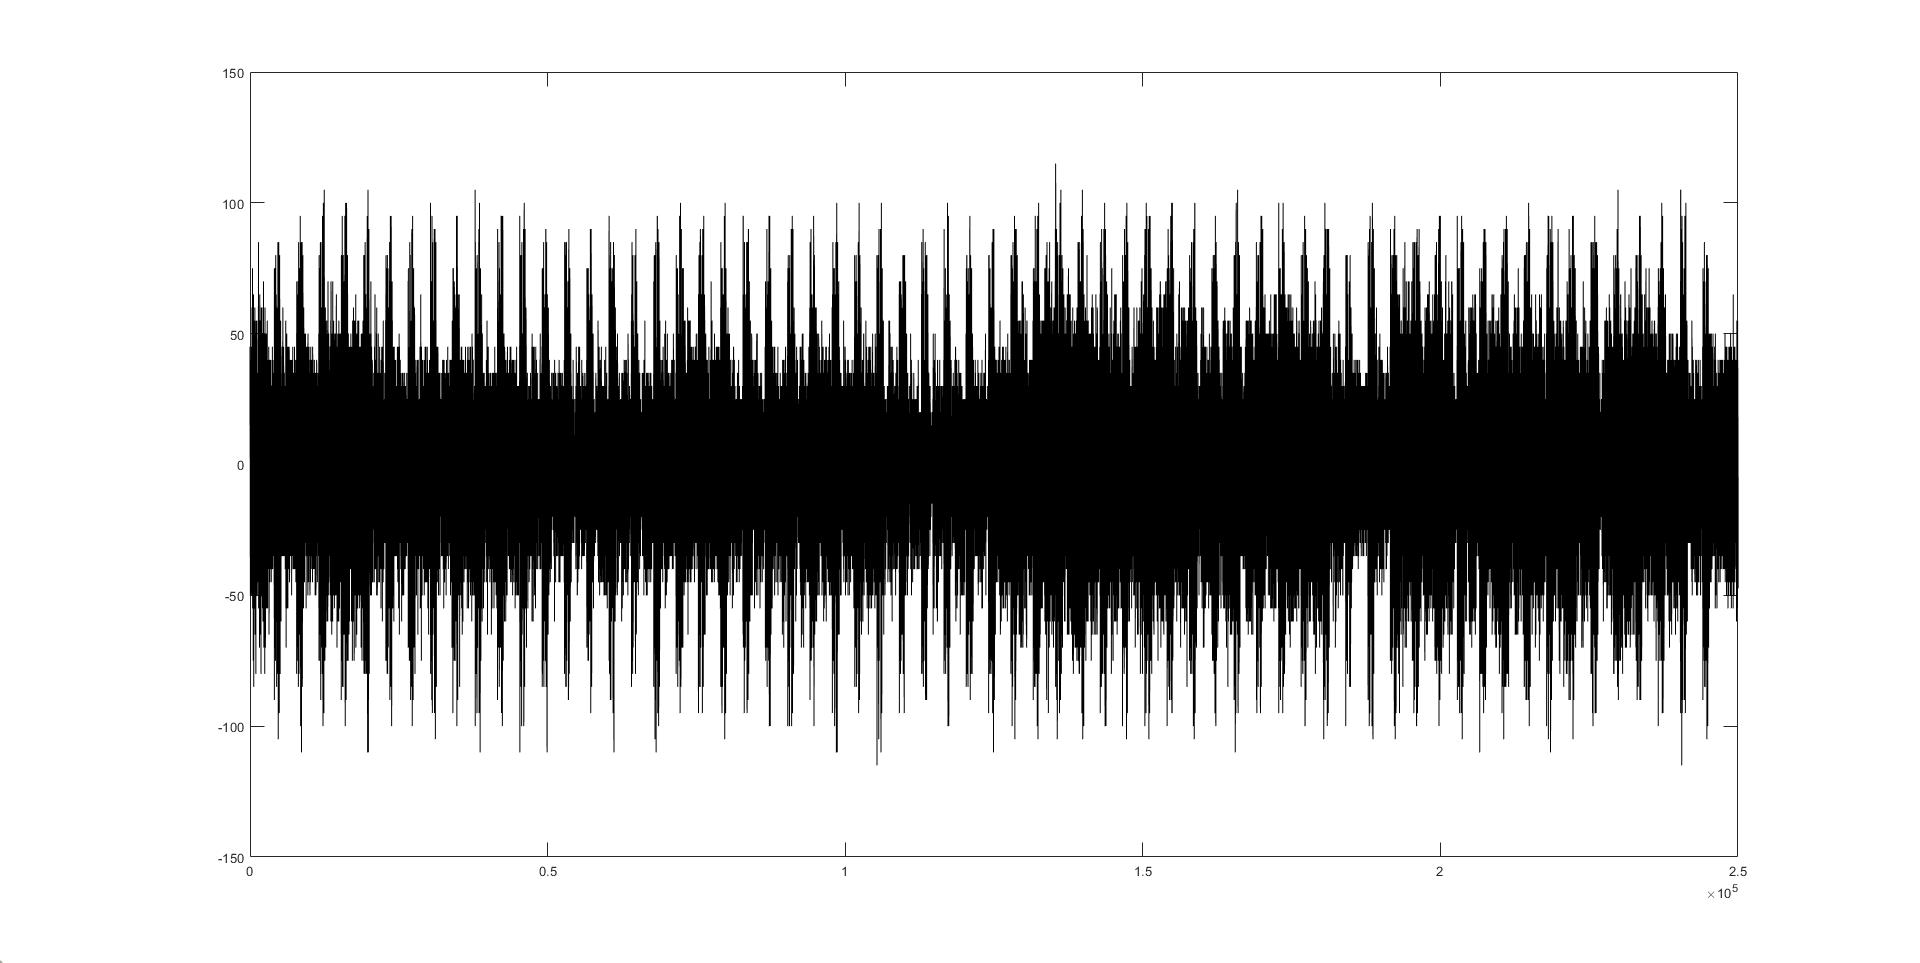
\includegraphics[width=230mm,scale=0.7]{g10s1.jpg}
\end{center}
\end{figure*}
\newpage
\section*{Τραγούδι: Chase the sun}
\section*{G11. Ιστόγραμμα δειγμάτων (DPCM) }
\begin{figure*}[h!]
 \begin{center}
 \advance\leftskip-6cm
  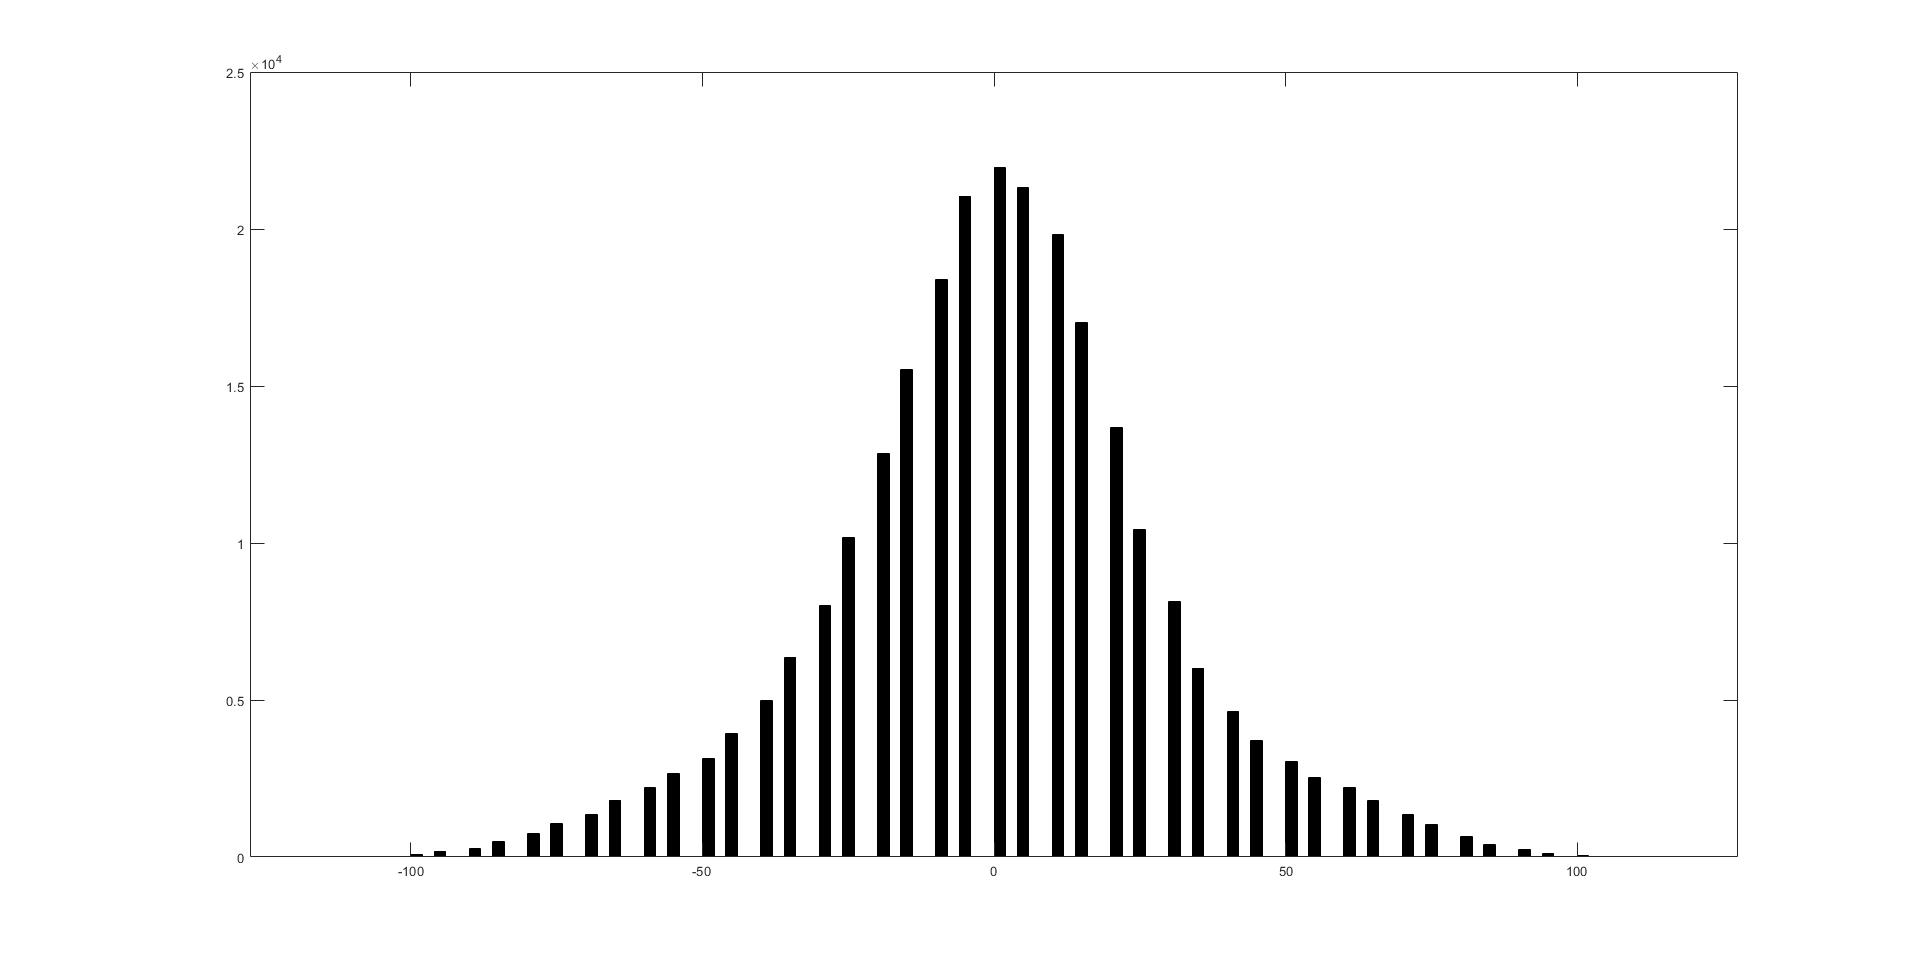
\includegraphics[width=230mm,scale=0.7]{g11s1.jpg}
\end{center}
\end{figure*}
\newpage
\section*{Τραγούδι: Chase the sun}
\section*{G12. Ιστόγραμμα διαφορών (DPCM) }
\begin{figure*}[h!]
 \begin{center}
 \advance\leftskip-6cm
  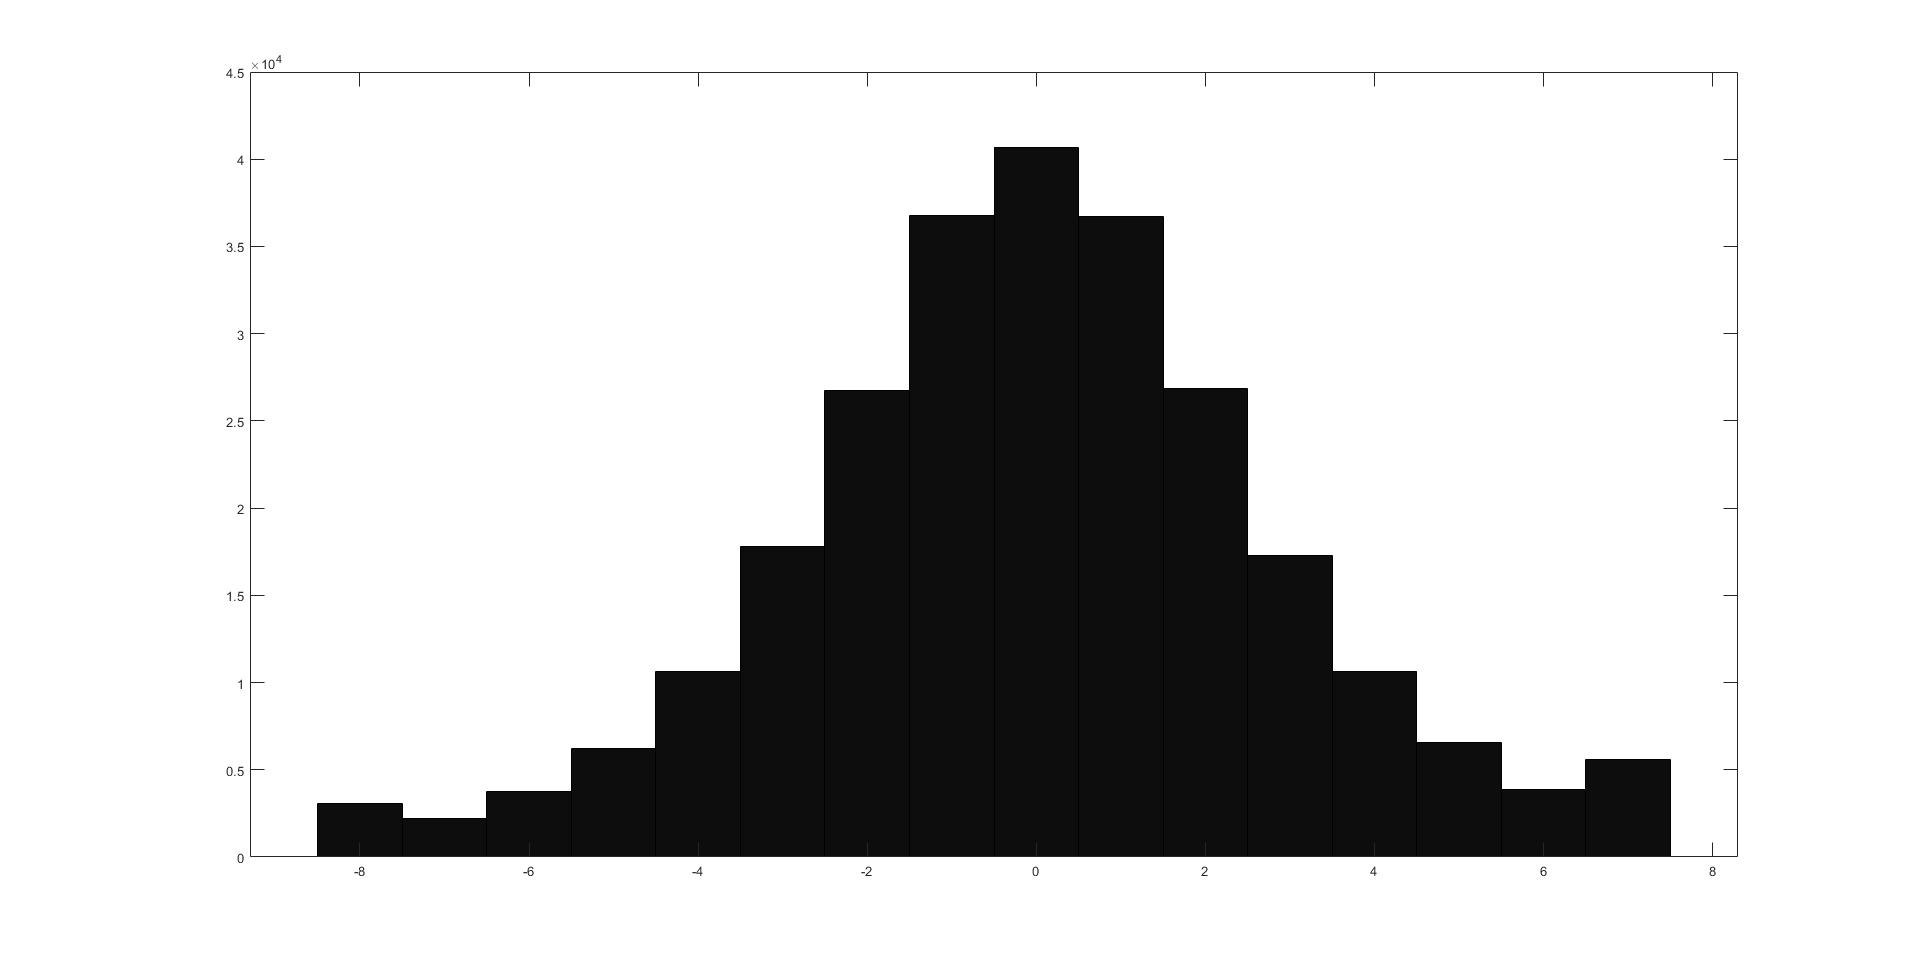
\includegraphics[width=230mm,scale=0.7]{g12s1.jpg}
\end{center}
\end{figure*}
\newpage
\section*{Τραγούδι: Sexy Love}
\section*{G13. Ιστόγραμμα δειγμάτων (AQDPCM) }
\begin{figure*}[h!]
 \begin{center}
 \advance\leftskip-6cm
  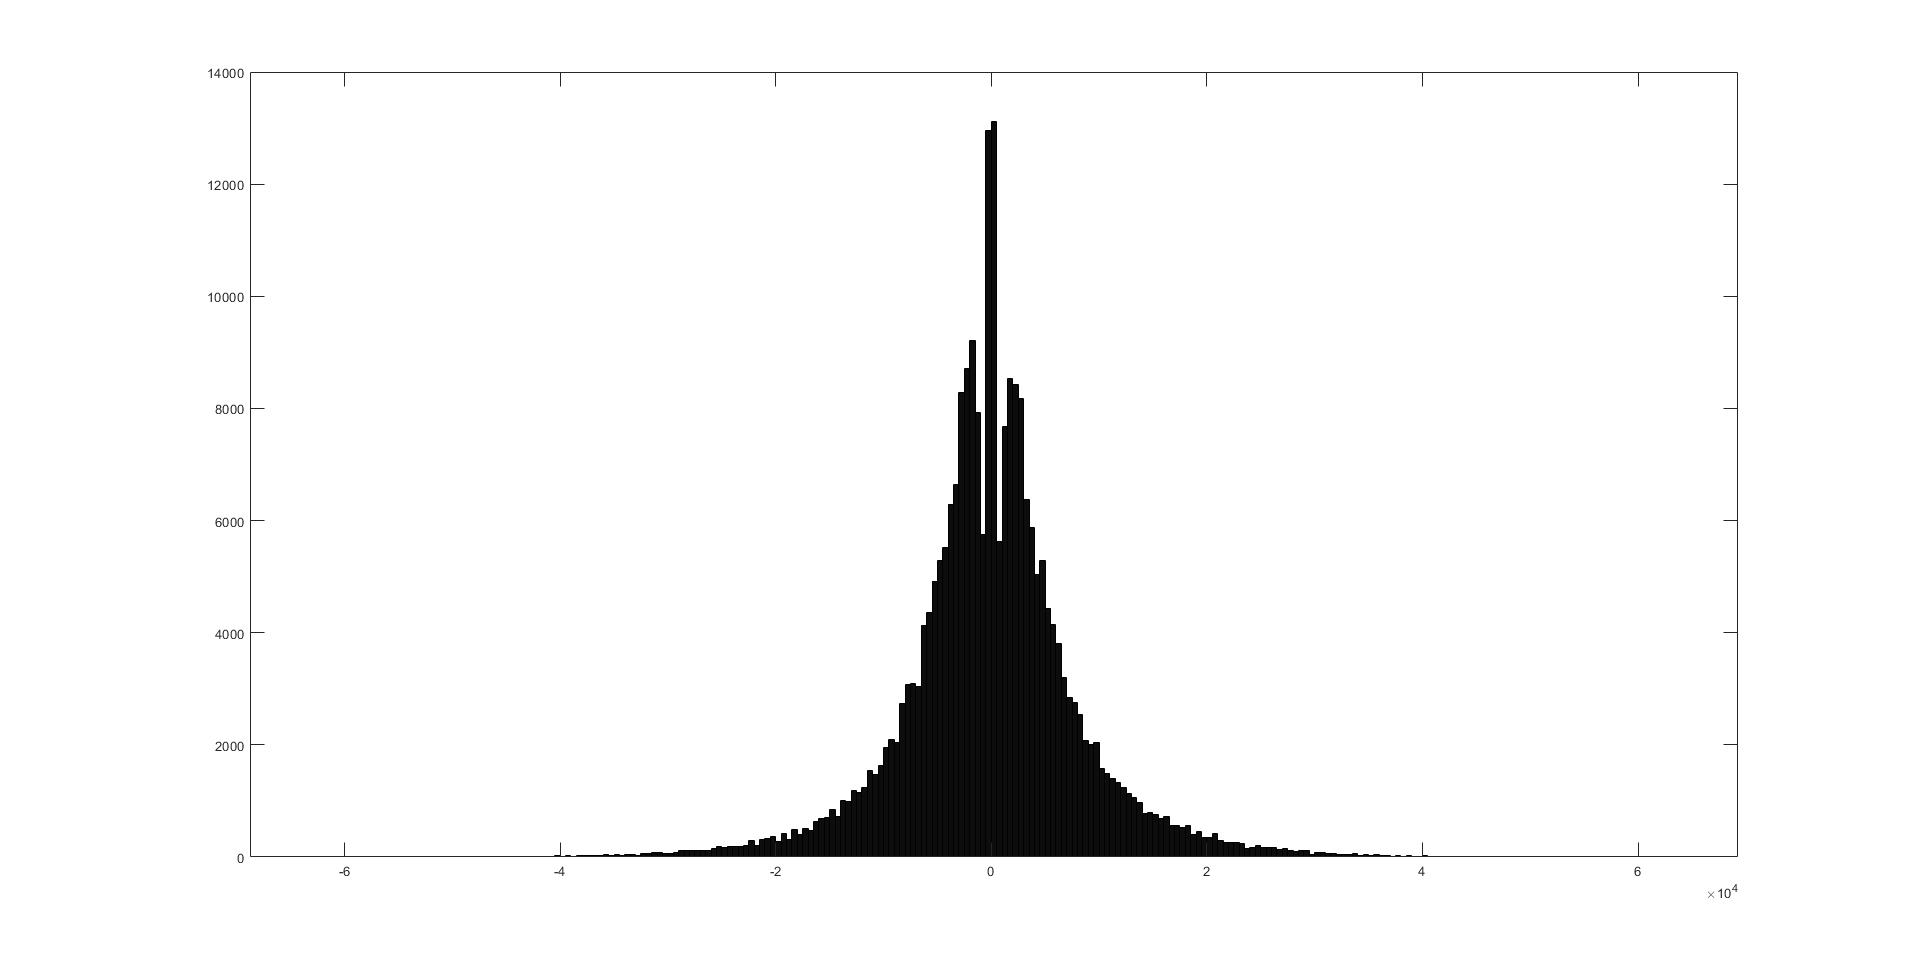
\includegraphics[width=230mm,scale=0.7]{g13s1.jpg}
\end{center}
\end{figure*}
\newpage
\section*{Τραγούδι: Sexy Love}
\section*{G14. Ιστόγραμμα διαφορών (AQDPCM) }
\begin{figure*}[h!]
 \begin{center}
 \advance\leftskip-6cm
  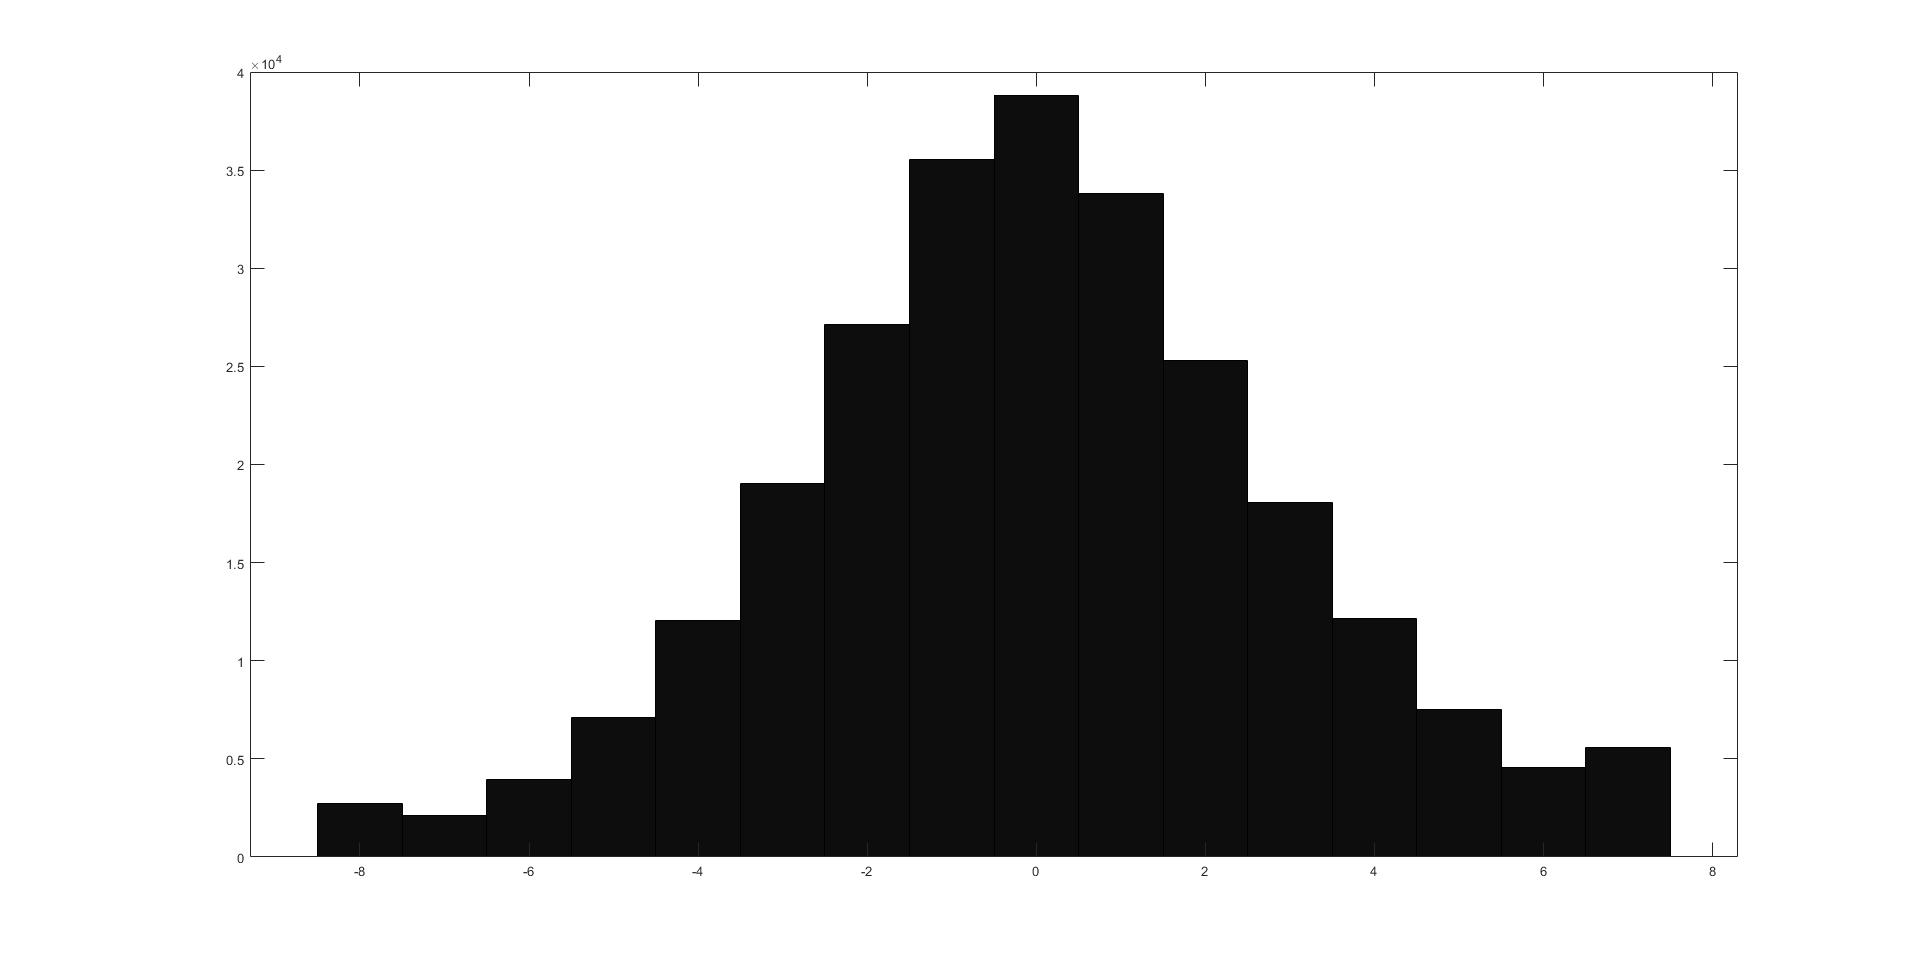
\includegraphics[width=230mm,scale=0.7]{g14s1.jpg}
\end{center}
\end{figure*}
\newpage
\section*{Τραγούδι: Sexy Love}
\section*{G15. Μέση τιμή κβαντιστή (AQDPCM) }
\begin{figure*}[h!]
 \begin{center}
 \advance\leftskip-6cm
  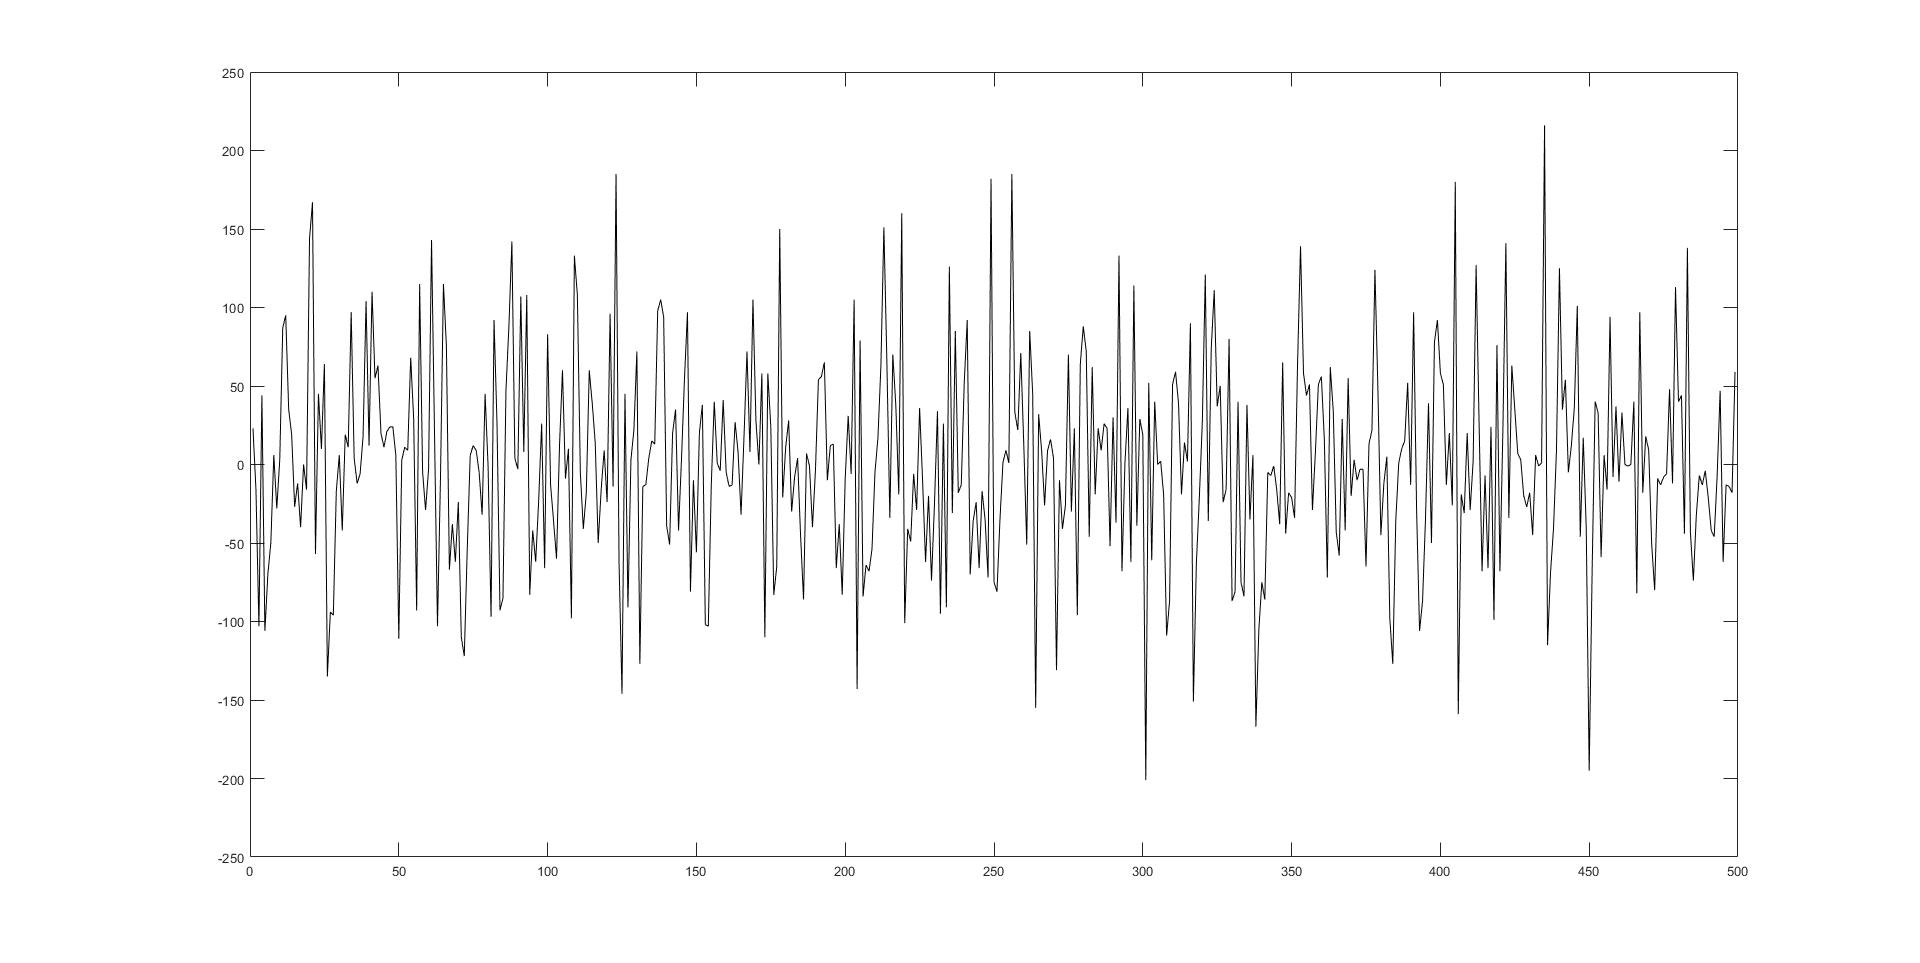
\includegraphics[width=230mm,scale=0.7]{g15s1.jpg}
\end{center}
\end{figure*}
\newpage
\section*{Τραγούδι: Sexy Love}
\section*{G16. Βήμα κβαντιστή (AQDPCM) }
\begin{figure*}[h!]
 \begin{center}
 \advance\leftskip-6cm
  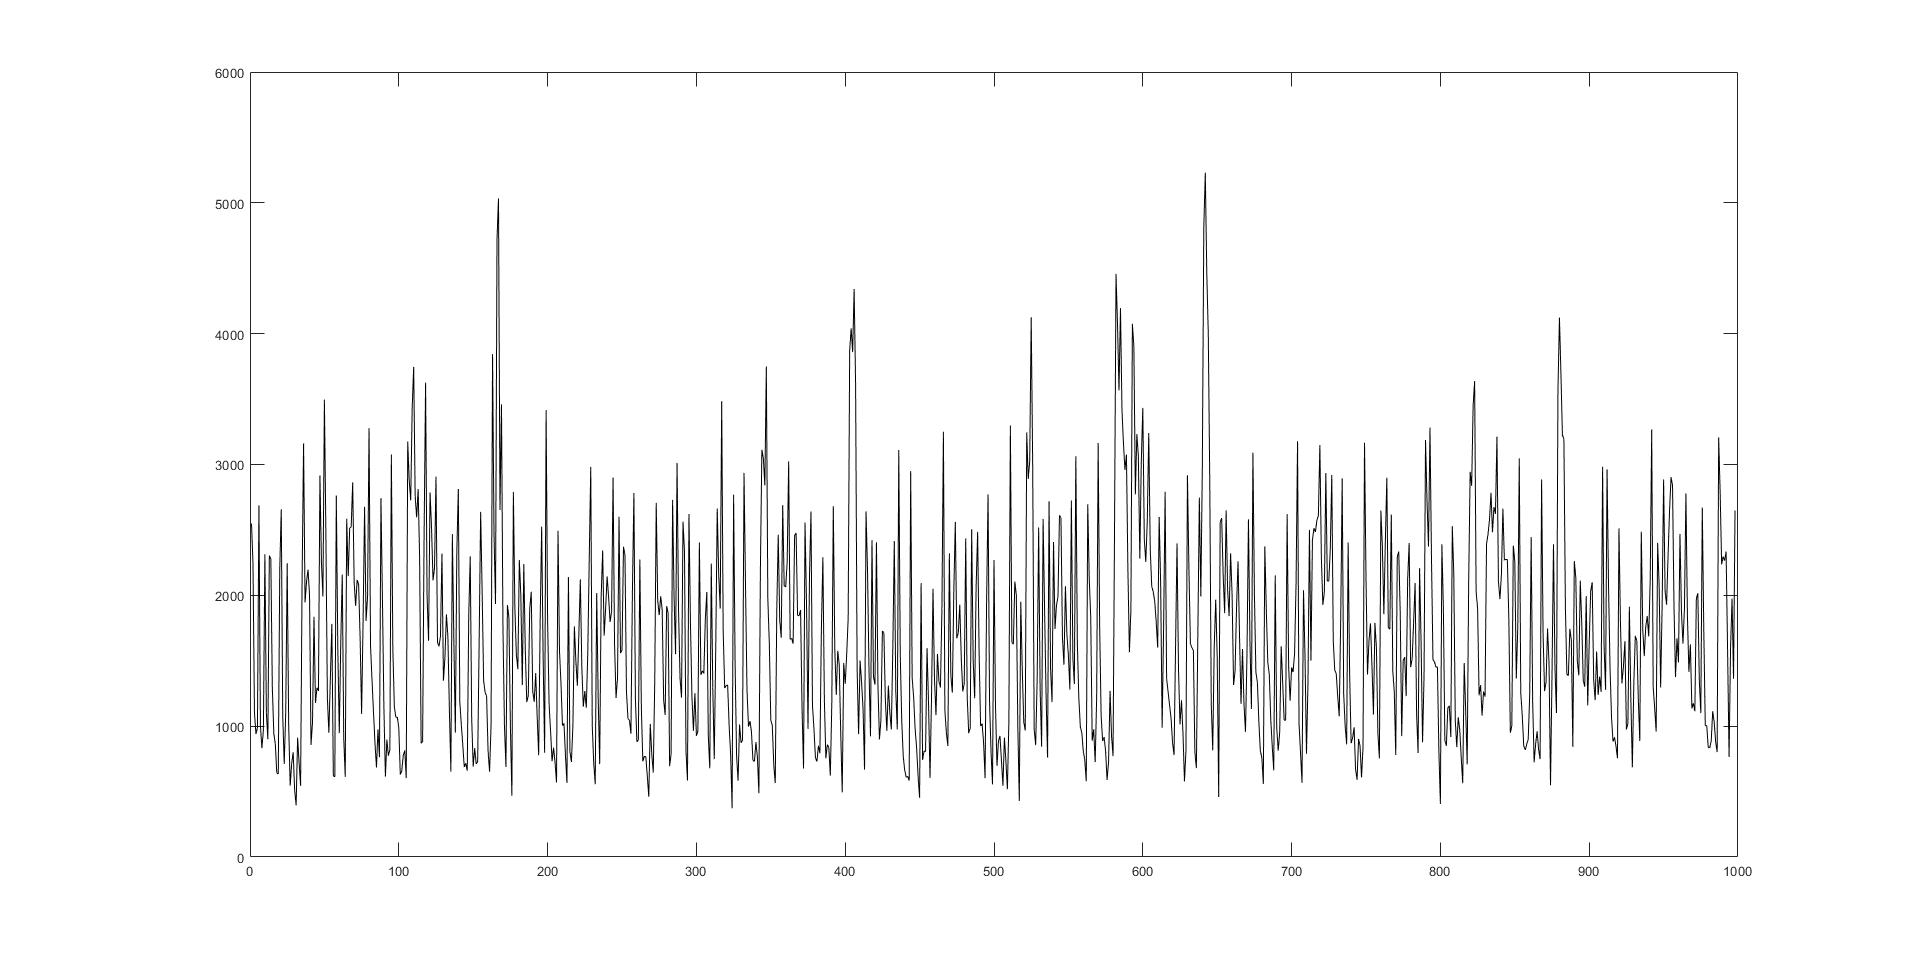
\includegraphics[width=230mm,scale=0.7]{g16s1.jpg}
\end{center}
\end{figure*}
\newpage
\section*{Τραγούδι: Theme from serpico}
\section*{G17. Μέση τιμή κβαντιστή (AQDPCM) }
\begin{figure*}[h!]
 \begin{center}
 \advance\leftskip-6cm
  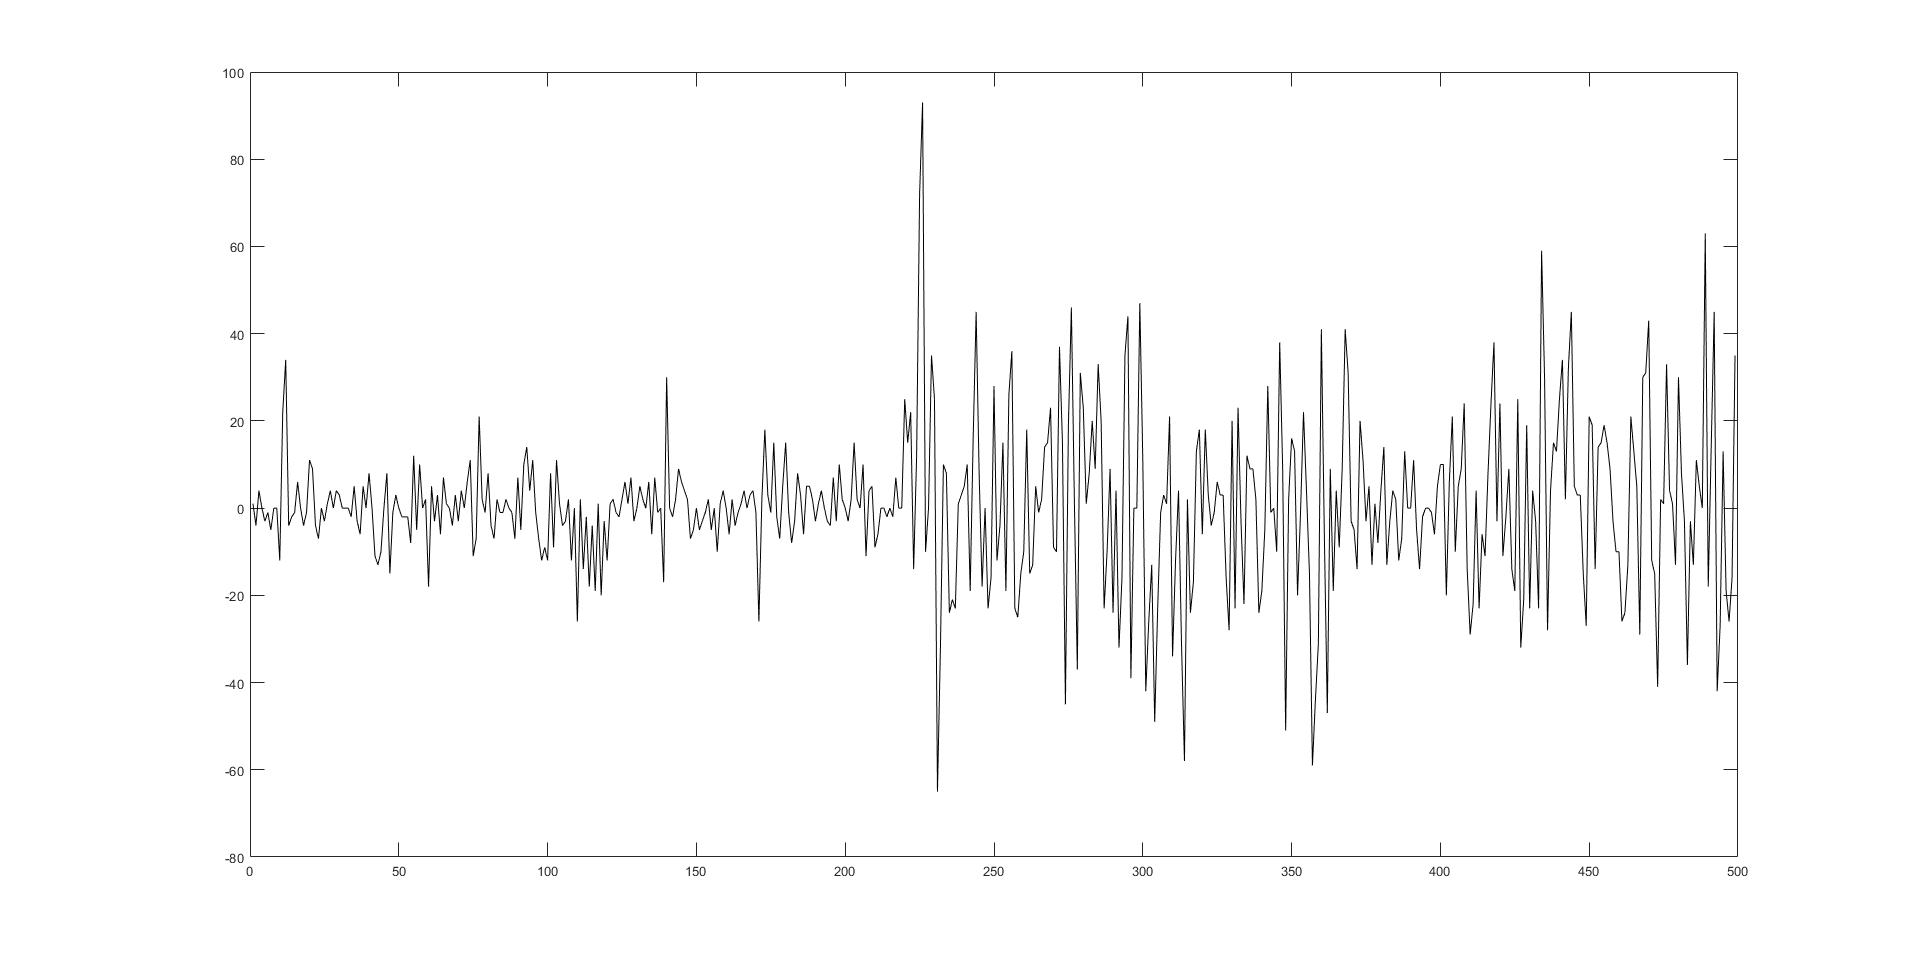
\includegraphics[width=230mm,scale=0.7]{g17s1.jpg}
\end{center}
\end{figure*}
\newpage
\section*{Τραγούδι: Theme from serpico}
\section*{G18. Μέση τιμή κβαντιστή (AQDPCM) }
\begin{figure*}[h!]
 \begin{center}
 \advance\leftskip-6cm
  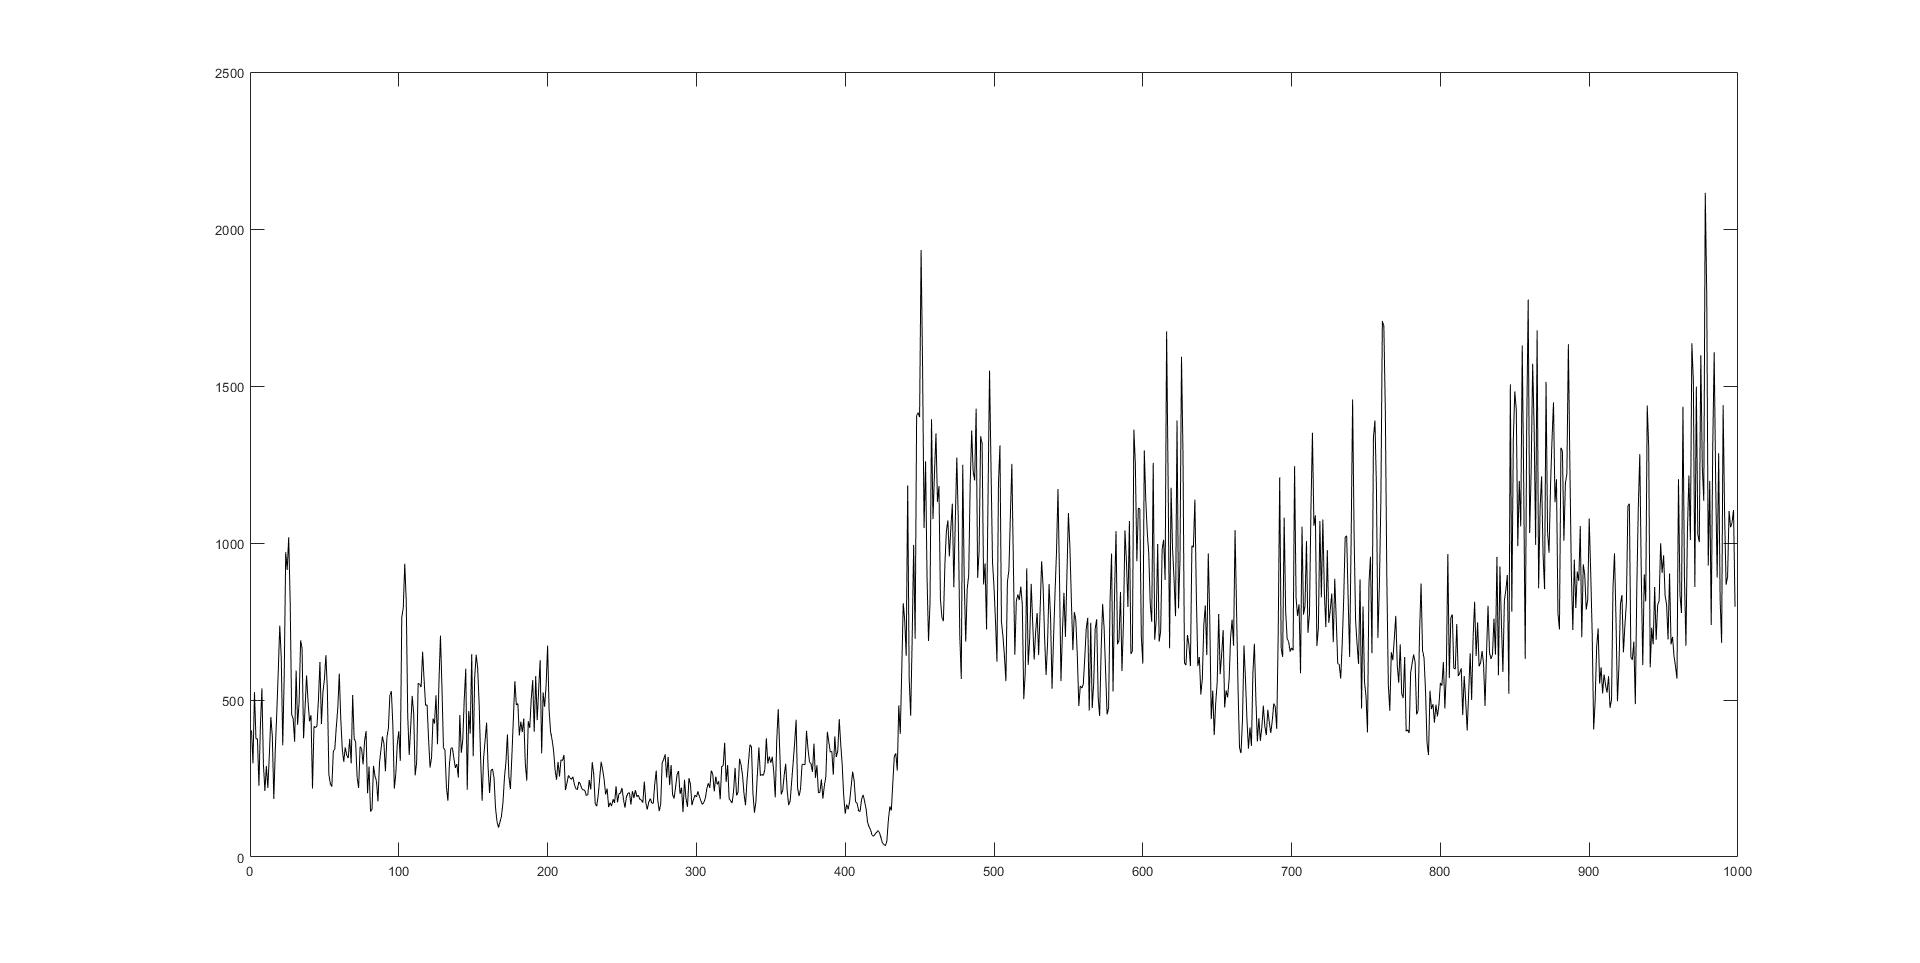
\includegraphics[width=230mm,scale=0.7]{g18s1.jpg}
\end{center}
\end{figure*}
\newpage
\section*{G21. Vehicle Engine run time }
\begin{figure*}[h!]
 \begin{center}
 \advance\leftskip-6cm
  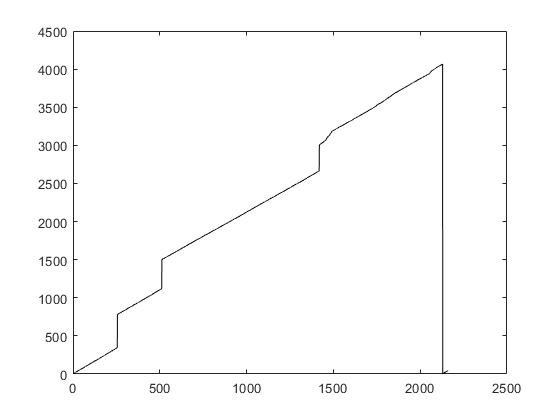
\includegraphics[width=230mm,scale=0.7]{g21s1.jpg}
\end{center}
\end{figure*}
\newpage
\section*{G22. Vehicle Engine RPM }
\begin{figure*}[h!]
 \begin{center}
 \advance\leftskip-6cm
  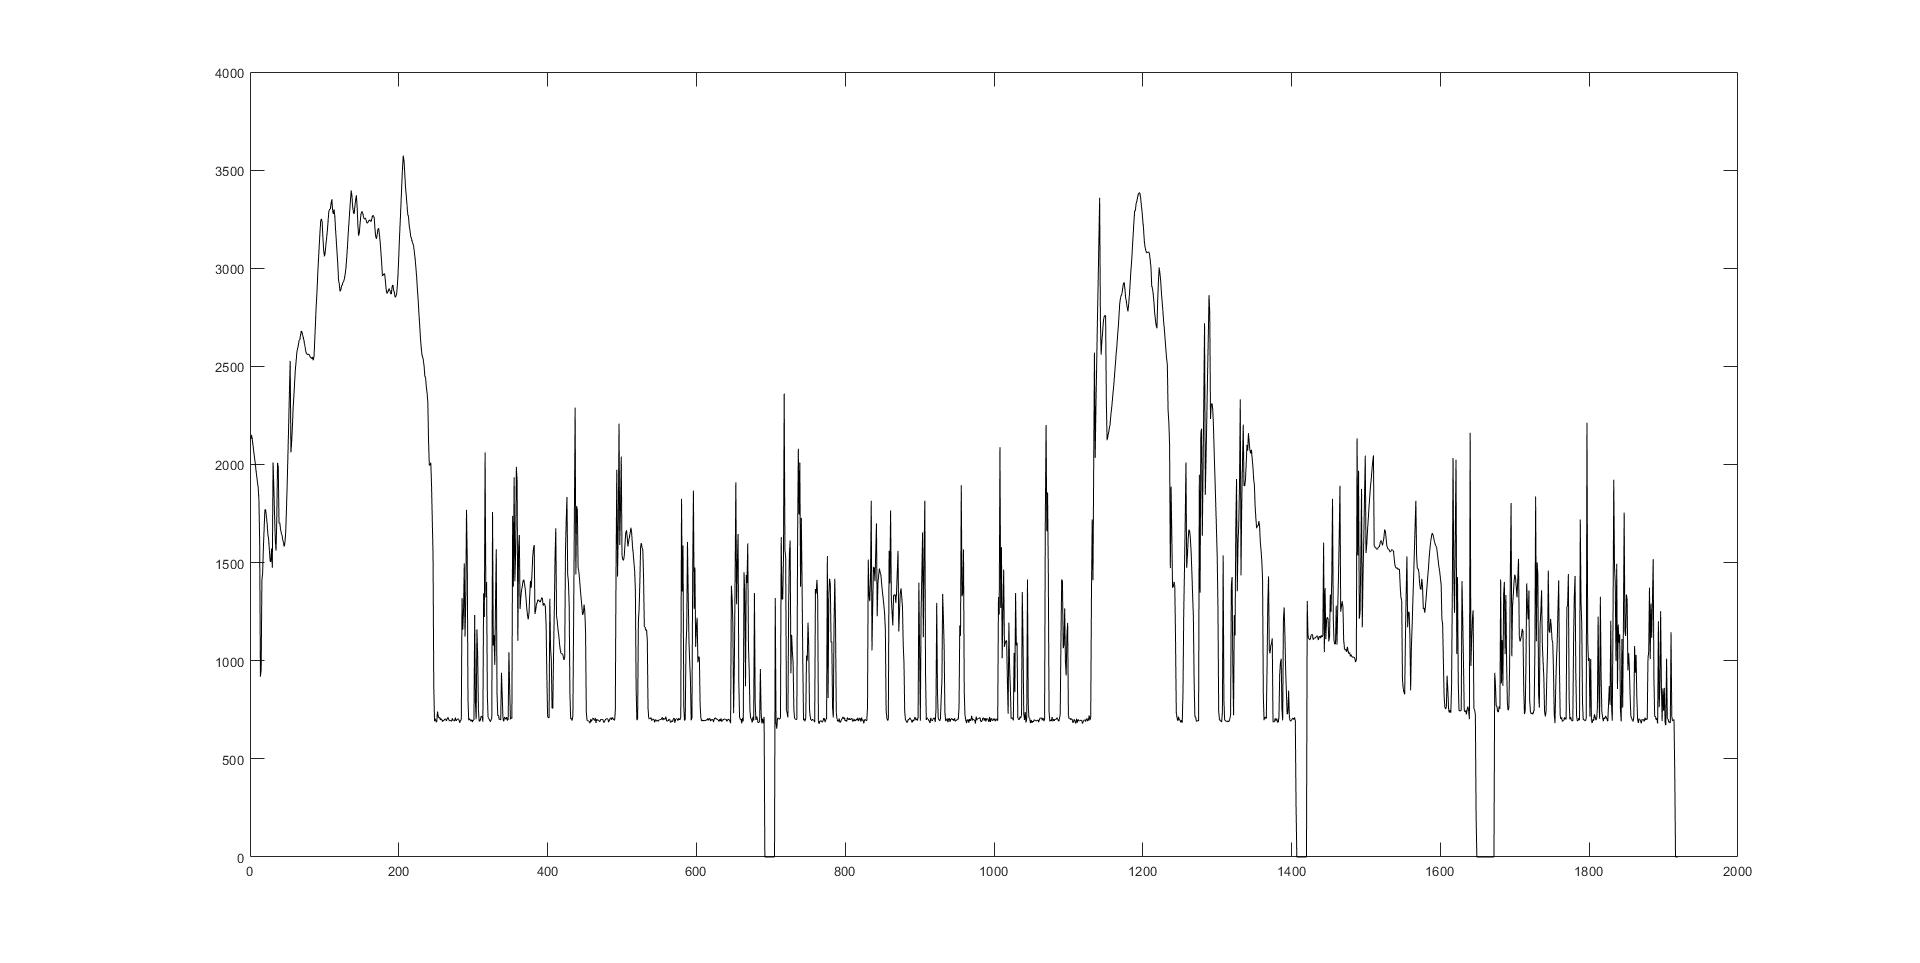
\includegraphics[width=230mm,scale=0.7]{g22s1.jpg}
\end{center}
\end{figure*}
\newpage
\section*{G23. Vehicle Speed }
\begin{figure*}[h!]
 \begin{center}
 \advance\leftskip-6cm
  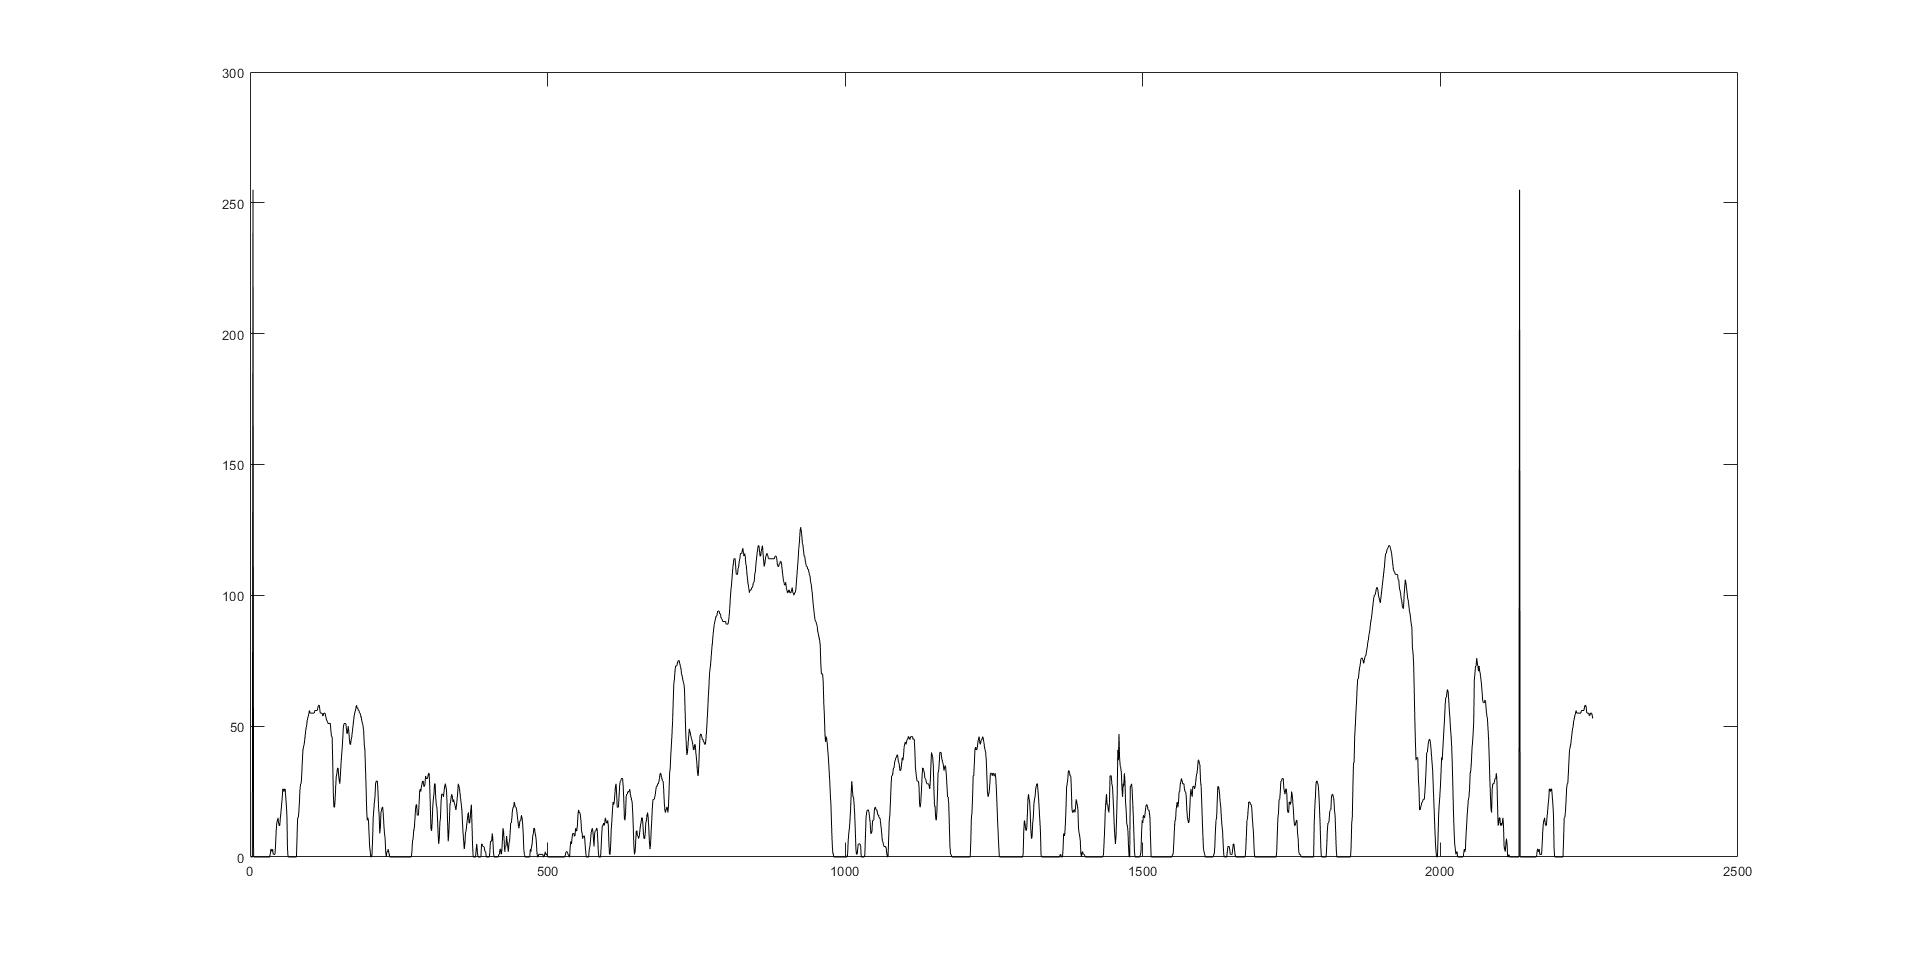
\includegraphics[width=230mm,scale=0.7]{g23s1.jpg}
\end{center}
\end{figure*}
\newpage
\section*{G24. Vehicle Intake air temperature }
\begin{figure*}[h!]
 \begin{center}
 \advance\leftskip-6cm
  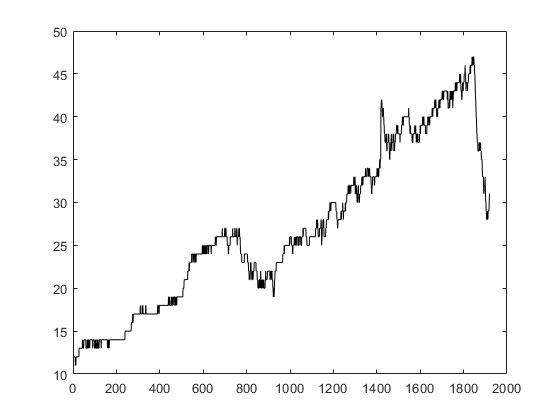
\includegraphics[width=230mm,scale=0.7]{g24s1.jpg}
\end{center}
\end{figure*}
\newpage
\section*{G25. Vehicle Throttle position }
\begin{figure*}[h!]
 \begin{center}
 \advance\leftskip-6cm
  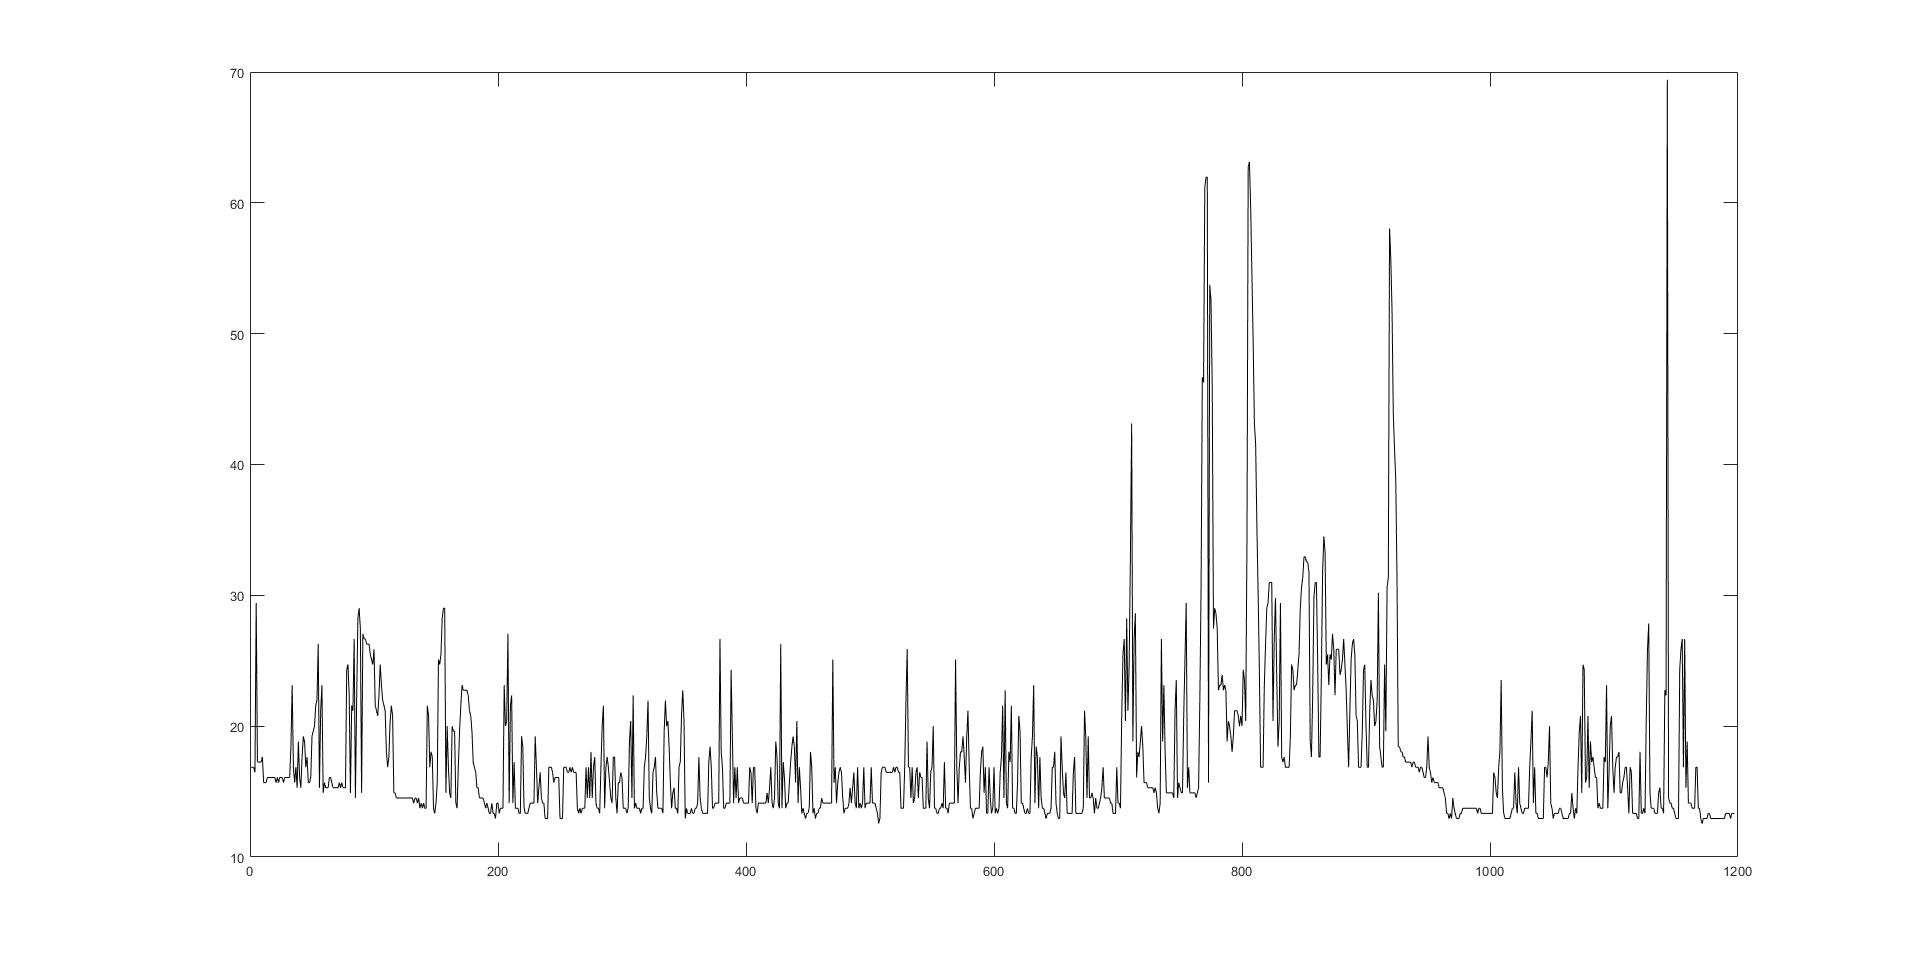
\includegraphics[width=230mm,scale=0.7]{g25s1.jpg}
\end{center}
\end{figure*}
\newpage
\section*{G26. Vehicle Coolant temperature }
\begin{figure*}[h!]
 \begin{center}
 \advance\leftskip-6cm
  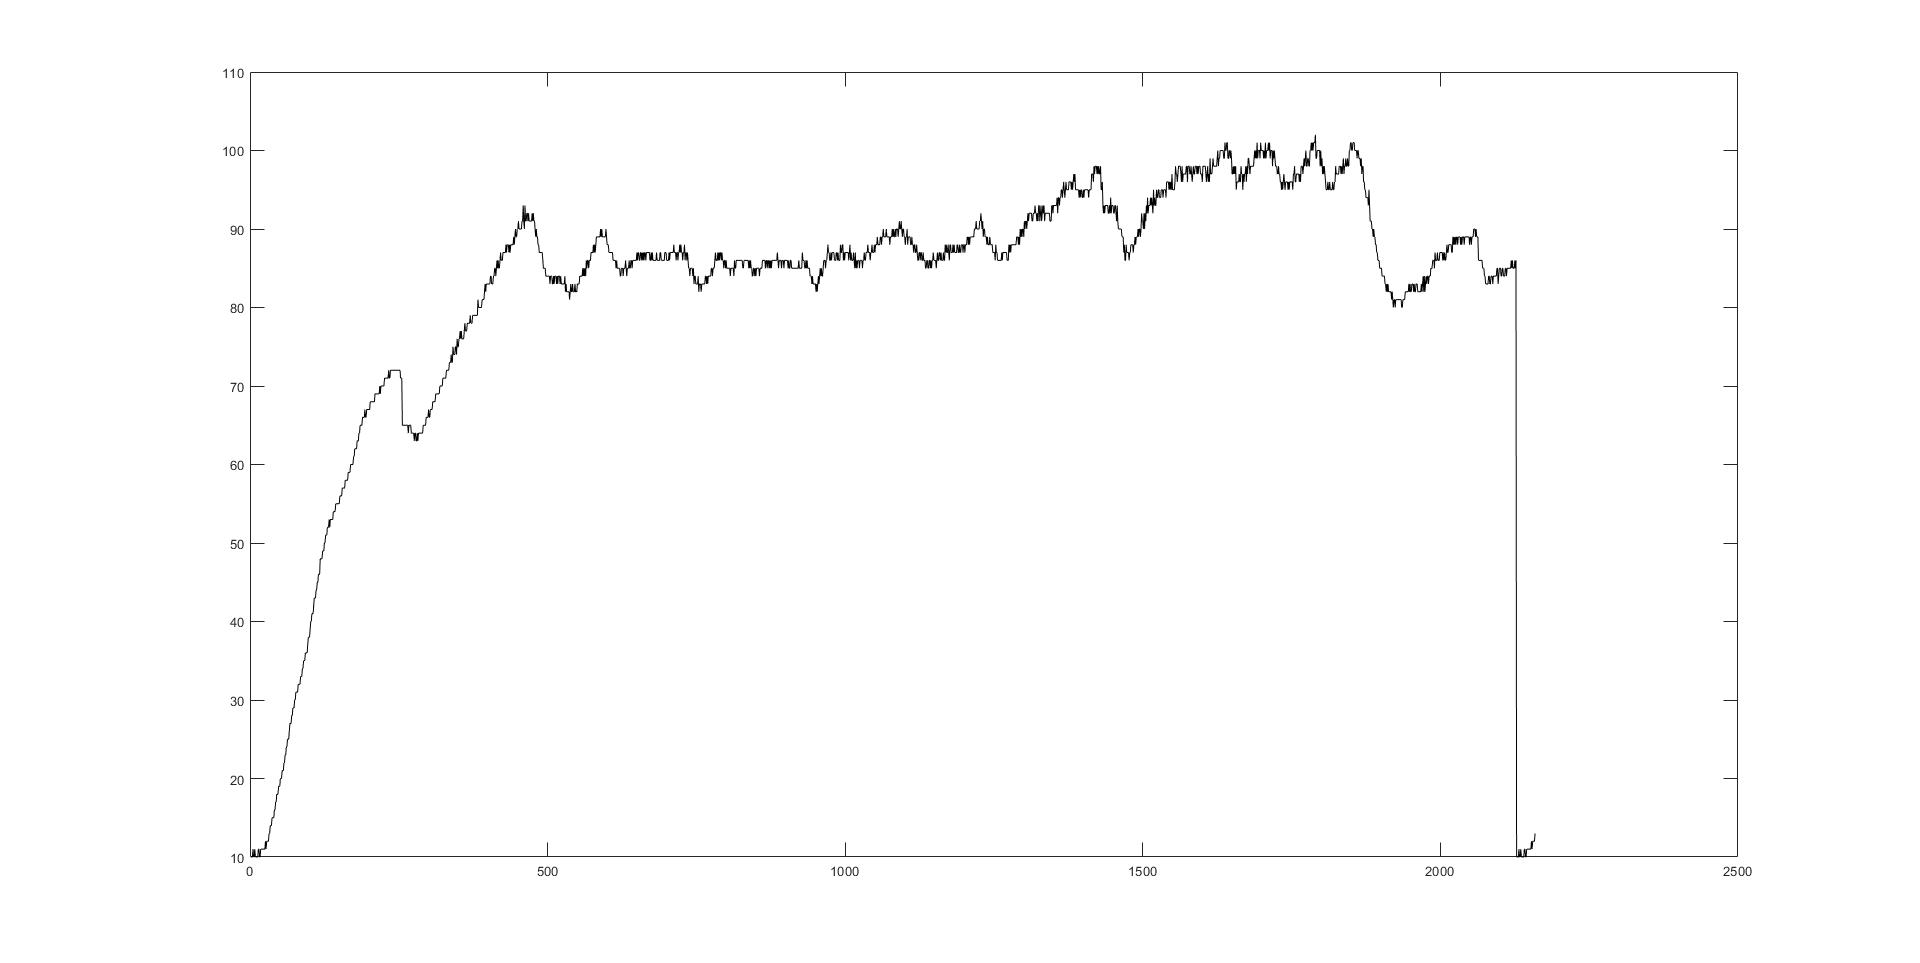
\includegraphics[width=230mm,scale=0.7]{g26s1.jpg}
\end{center}
\end{figure*}
\end{document}